\documentclass[a4paper, article, 14pt]{extarticle}

% Подключаем главный пакет со всем необходимым
\usepackage{spbudiploma_tempora}

% Пакеты по желанию (самые распространенные)
% Хитрые мат. символы
\usepackage{euscript}
% Таблицы
\usepackage{longtable}
\usepackage{makecell}
% Картинки (можно встявлять даже pdf)
\usepackage[pdftex]{graphicx}

\usepackage{amsthm, amssymb, amsmath}
\usepackage{textcomp}


%%% Здесь то, что было добавлено мной (sasha.menkeev@mail.ru)

% Поменьше пространства между элементами списка, а также снизу и сверху от него
\usepackage[shortlabels]{enumitem}
\setlist{itemsep=2pt,parsep=2pt,topsep=4pt,partopsep=2pt}

\usepackage{listings}
\usepackage{color}

\definecolor{dkgreen}{rgb}{0,0.6,0}
\definecolor{gray}{rgb}{0.5,0.5,0.5}
\definecolor{mauve}{rgb}{0.58,0,0.82}
\definecolor{lbcolor}{RGB}{245,245,245}
\definecolor{green}{RGB}{62,125,74}
\definecolor{yellowish}{RGB}{193,178,138}

\lstset{
    backgroundcolor=\color{lbcolor},
    frame=tb,
    language=[Sharp]C,
    escapeinside=``,
    aboveskip=3mm,
    belowskip=3mm,
    showstringspaces=false,
    columns=flexible,
    basicstyle={\small\ttfamily},
    numbers=left,
    stepnumber=1,
    firstnumber=auto,
    numberfirstline=true
    numberstyle=\tiny\color{gray},
    keywordstyle=\color{blue},
    commentstyle=\color{dkgreen},
    stringstyle=\color{mauve},
    breaklines=true,
    breakatwhitespace=true,
    tabsize=3
}

%%%

\begin{document}

% Титульник в файле titlepage.tex
\newgeometry{left=30mm, top=20mm, right=15mm, bottom=20mm, nohead, nofoot}
\begin{titlepage}
\begin{center}

\textbf{Санкт--Петербургский}
\textbf{государственный университет}

\vspace{35mm}

\textbf{\textit{\large Менкеев Александр Саналович}} \\[8mm]
% Название
\textbf{\large Выпускная квалификационная работа}\\[3mm]
\textbf{\textit{\large Применение методов нейроэволюции при разработке мобильной игры с процедурной генерацией контента}}

\vspace{20mm}
Уровень образования: бакалавриат\\
Направление: 02.03.02 «Фундаментальная информатика и информационные технологии»\\
Основная образовательная программа СВ.5003.2020 
«Программирование и информационные технологии»\\[10mm]


% Научный руководитель, рецензент
\begin{flushright}
\begin{minipage}[t]{0.56\textwidth}
{Научный руководитель:} \\
доцент, кафедра теории систем управления электрофизической аппаратурой, к.ф. - м.н.\\
Головкина Анна Геннадьевна

\vspace{6mm}

{Рецензент:} \\
доцент, кафедра технологии\\ программирования, к.т.н.\\ Блеканов Иван Станиславович
\end{minipage}
\end{flushright}

\vfill 

{Санкт-Петербург}
\par{\the\year{} г.}
\end{center}
\end{titlepage}
% Возвращаем настройки geometry обратно (то, что объявлено в преамбуле)
\restoregeometry
% Добавляем 1 к счетчику страниц ПОСЛЕ titlepage, чтобы исключить 
% влияние titlepage environment
\addtocounter{page}{1}


% Содержание
\tableofcontents
\pagebreak

%! suppress = LineBreak
\specialsection{Введение}

С тех пор как были изобретены компьютерные игры, количество человеко-месяцев, которые уходят на разработку успешной коммерческой игры, постоянно увеличивалось. Сейчас является нормой, что игра разрабатывается сотнями людей на протяжении года или даже дольше. Вследствие этого всё меньше игр являются прибыльными и всё меньше разработчиков способны выпустить собственную игру, что в свою очередь, приводит к меньшей готовности рисковать и меньшему разнообразию на рынке игр. Процедурная генерация контента способна частично устранить эту проблему, ведь многие из дорогостоящих сотрудников, необходимых в этом процессе являются дизайнерами и художниками, а не программистами. Компания по разработке игр, которая смогла бы заменить некоторых художников и дизайнеров алгоритмами, получила бы конкурентное преимущество, поскольку была бы способна производить игры быстрее и дешевле, сохраняя при этом качество.

Более того, методы процедурной генерации способны значительно повысить среднее игровое время. Ведь если игра реализует алгоритм, способный генерировать игровой контент со скоростью, с которой он потребляется, то в принципе нет причин, почему она должна завершаться. У игроков не будут заканчиваться уровни для прохождения, области для исследования, оружие для использования, персонажи для взаимодействия.

Ещё более захватывающей является идея игрового контента, который бы соответствовал вкусам игрока. Используя нейронные сети и методы их эволюции, можно создать систему процедурной генерации контента, которая бы подстраивалась под предпочтения игрока. 

Очевидно, чтобы генерировать что-то, нужно знать что именно требуется получить. Какие свойства артефакта являются желаемыми? Какие будут нарушать игровой процесс и их следует исключить? Какой алгоритм использовать?

Данная работа посвящена методам процедурной генерации контента на примере генерации игрового оружия. 

\pagebreak

\specialsection{Постановка задачи}

Целью данной работы является разработка программного инструмента, интегрированного в игровой движок Unity и предназначенного для процедурной генерации игрового оружия с уникальными траекториями снарядов.

Разрабатываемая система призвана облегчить разработку 2D игр в жанре шутеры и должна удовлетворять следующим требованиям:
\begin{enumerate}
    \item Система должна иметь достаточное количество настраиваемых параметров оружия, чтобы пользователь мог генерировать именно то, что ему нужно.
    \item Система не должна требовать больших усилий со стороны пользователя для генерации оружия.
    \item Система должна иметь качественный пользовательский интерфейс, работающий внутри Unity.
    \item Система должна иметь демонстрационные игровые сцены, показывающие возможные сценарии использования.
\end{enumerate}

\vspace{5mm}

Целью также является создание прототипа мобильной 2D игры, которая бы использовала эту систему. Требования для игры:
\begin{enumerate}
    \item Интерфейс, позволяющий игроку выбирать или отказываться от оружия, а также редактировать некоторые его параметры.
    \item Два джойстика: один для движения, другой для стрельбы.
    \item Наличие стреляющего врага, при этом вражеские снаряды и снаряды игрока должны иметь возможность сталкиваться.
\end{enumerate}

\pagebreak

\specialsection{Обзор литературы}





\pagebreak

\section{Обзор существующих решений}


\pagebreak

%! suppress = LineBreak
\section{Оружие, основанное на системе частиц}\label{sec:WeaponIdea}

Оружие, генерируемое системой, основано на идее из программы NEAT Particles\cite{s2,s3}. Каждое оружие содержит в себе нейронную сеть (Рисунок~\ref{Weapon}). Каждый кадр анимации каждая частица, выпущенная из оружия, подает на вход в нейронную сеть:

\begin{enumerate}
    \item {\small \textbf{RelativePos.x}} -- координата $x$ текущего положения частицы относительно точки выстрела.
    \item {\small \textbf{RelativePos.y}} -- координата $y$ текущего положения частицы относительно точки выстрела.
    \item {\small \textbf{DistanceFromOrigin}} -- расстояние от точки выстрела.
\end{enumerate}

 После этого нейронная сеть активируется и выводит для этого анимационного кадра:

\begin{enumerate}
    \item {\small \textbf{x}} -- координата $x$ вектора скорости или силы, приложенной к частице.
    \item {\small \textbf{y}} -- координата $y$ вектора скорости или силы, приложенной к частице.
    \item {\small \textbf{hue}} -- компонента цвета частицы в модели HSV\@.
    \item {\small \textbf{maxSpeed}} -- максимальная скорость частицы.
    \item {\small \textbf{force}} -- длина вектора скорости или силы, приложенной к частице.
\end{enumerate}


\begin{figure}[ht]
    \begin{center}
        \scalebox{0.17}{
            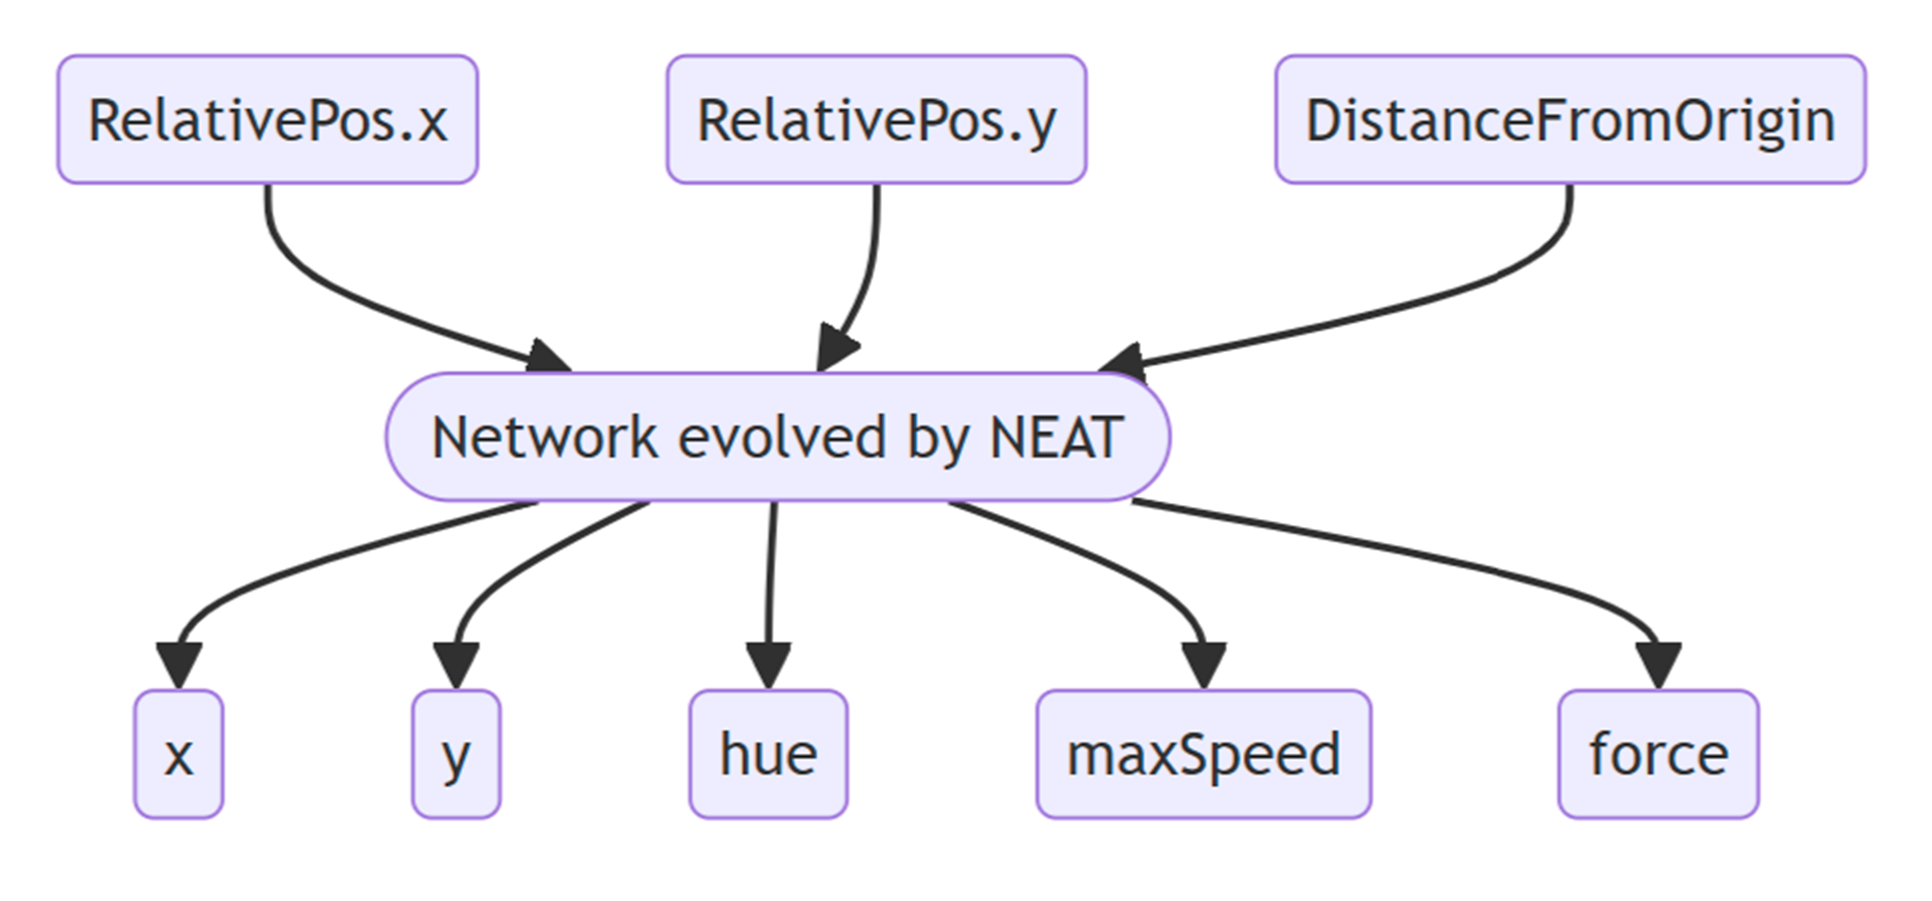
\includegraphics{images/GenIdea}
        }

        \caption{
            \label{Weapon}
            Как нейронная сеть управляет снарядами.}
    \end {center}
\end {figure}


Поскольку оружие представляется нейронной сетью, можно генерировать новое оружие, изменяя веса или топологию нейронной сети. Выбор алгоритма для этого обосновывается в следующей главе.

\pagebreak

%! suppress = LineBreak
%! suppress = MissingLabel
\section{Методы эволюции нейронных сетей}\label{sec:evolutionMethods}

Существует множество алгоритмов для эволюции нейронных сетей. Они классифицируются по схемам кодирования и тому, модифицируют ли они веса, топологию или и то, и другое. Однако не все они пользуются популярностью и имеют хорошие библиотеки с реализацией. Можно выделить два алгоритма NEAT\cite{s1} и HyperNEAT\cite{s1}, которые находят своё применение до сих пор и имеют регулярно обновляемые библиотеки.

\subsection{NEAT}

Название этого алгоритма расшифровывается как нейроэволюция расширяющихся топологий (NeuroEvolution of Augmenting Topologies). Это метод, предназначенный для эволюции искусственных нейронных сетей с помощью генетического алгоритма. Главная идея NEAT заключается в том, что эволюцию наиболее эффективно начинать с маленьких, простых сетей, которые постепенно становятся всё более сложными с каждым поколением.

Алгоритм основан на трех ключевых принципах. Во-первых, для того, чтобы позволить структурам нейронных сетей усложняться с течением поколений, необходим метод отслеживания того, какой ген является каким. В противном случае в последующих поколениях будет неясно, какая особь с какой совместима и как их гены должны быть объединены для получения потомства. NEAT решает эту проблему, присваивая уникальную историческую метку каждому новому элементу структуры сети, который появляется в результате структурной мутации. Историческая метка – это число, присвоенное каждому гену в соответствии с порядком его появления в ходе эволюции. Эти числа наследуются без изменений во время скрещиваний и позволяют NEAT выполнять скрещивание без необходимости трудоемкого топологического анализа. Таким образом геномы различной организации и размеров остаются совместимыми на протяжении всей эволюции, что решает ранее открытую проблему сопоставления различных топологий в эволюционирующей популяции. 

Во-вторых, NEAT разделяет популяцию на виды таким образом, что отдельные особи конкурируют в основном внутри своих собственных ниш, а не с популяцией в целом. Благодаря этому топологические инновации защищены и имеют время оптимизировать свою структуру, прежде чем конкурировать с другими нишами в популяции. NEAT использует исторические метки на генах, чтобы определить, к какому виду принадлежат различные особи. 

В-третьих, в отличие от других существующих систем эволюции нейронный сетей алгоритм NEAT начинается с однородной популяции простых сетей без скрытых узлов. Возникает новая топологическая структура по мере того, как происходят структурные мутации, и выживают только те структуры, которые признаны полезными в результате оценки функцией приспособленности. Таким образом, NEAT выполняет поиск топологических структур, начиная с самых простых, и находит оптимальную структуру для решения задачи.\\
%
Плюсы алгоритма:
\begin{enumerate}[--]
    \item Наличие актуальных библиотек с реализацией на разных языках программирования: C\#, C++, Python и другие.
    \item Операции мутации и скрещивания применяются не только к весам, но и к топологии нейронной сети.
    \item Подходит для трудно формализируемых задач, где функция потерь и функция приспособленности могут быть не определены.
\end{enumerate}
%
Минусы алгоритма:
\begin{enumerate}[--]
    \item Медленно сводится к оптимальному решению, если условия задачи очень сложны. 
    \item Плохо масштабируется из-за прямой схемы кодирования. Эффективно работает только с нейронными сетями малого размера, у которых меньше 200 узлов. 
\end{enumerate}

\subsection{HyperNEAT}

Полное название этого алгоритма можно перевести как нейроэволюция расширяющихся топологий, основанная на гиперкубе (Hypercube-based NeuroEvolution of Augmenting Topologies). HyperNEAT является дополнением NEAT и использует непрямую схему кодирования нейронных сетей для решения проблемы плохой масштабируемости.

Для непрямого кодирования используются субстрат и сети, производящие составные паттерны:

\begin{enumerate}[label=\textbullet]
    \item Субстрат -- это некоторое геометрическое упорядочивание узлов нейронной сети. Самый простой вариант такого упорядочивания -- решетка, где каждая отдельная точка $(x,y)$ является узлом (Рисунок~\ref{SubstratConfig}). 
    
    \begin{figure}[ht]
        \begin{center}
            \scalebox{0.4}{
                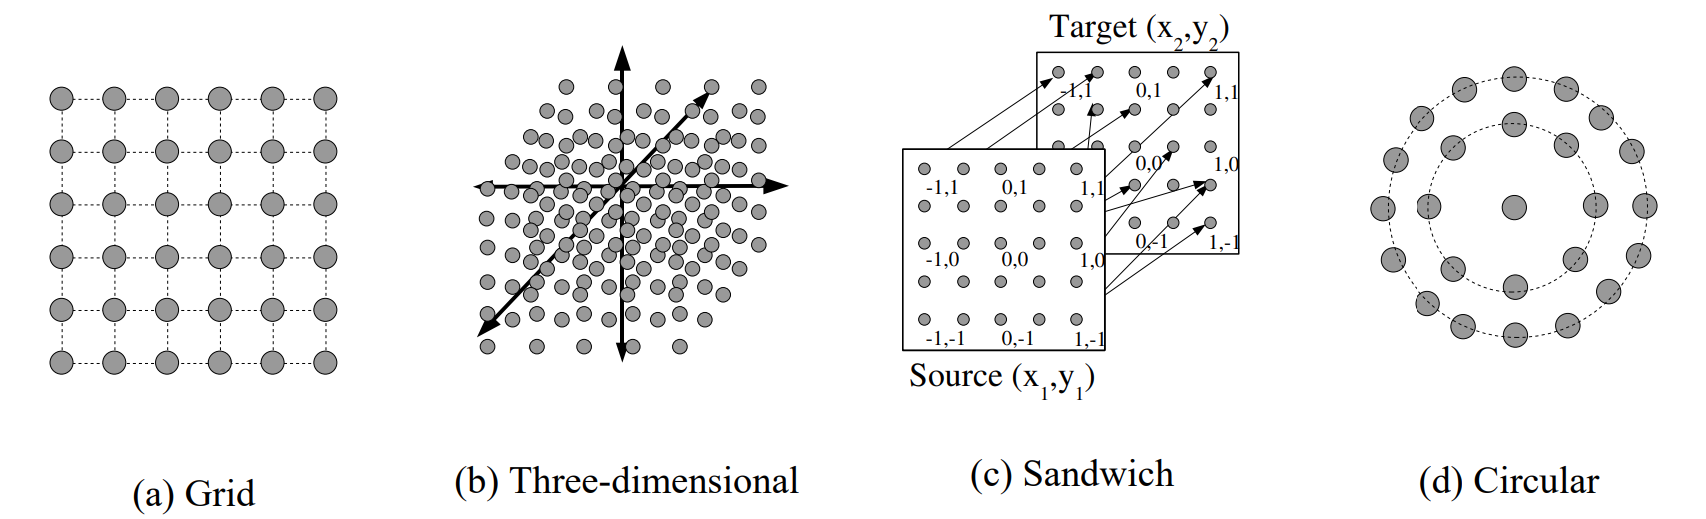
\includegraphics{images/SubstratConfig}
            }
    
            \caption{
                \label{SubstratConfig}
                Варианты субстратов.}
        \end {center}
    \end {figure}
    
    \item Сети, производящие составные паттерны (Compositional pattern-producing networks, далее – CPPN) -- это разновидность искусственных нейронных сетей. Основная особенность CPPN в том, что в их узлах могут использоваться разные функции активации. Выбор конкретного множества функций активации зависит от желаемых паттернов и закономерностей (Рисунок~\ref{CPPNvsANN}).
    \begin{figure}[ht]
        \begin{center}
            \scalebox{0.28}{
                \includegraphics{images/СPPNvsANN}
            }

            \caption{
                \label{CPPNvsANN}
                Разница между обычной нейронной сетью и CPPN.}
        \end {center}
    \end {figure}
\end{enumerate}



Алгоритм получения нейронной сети из субстрата описывается следующим образом (Рисунок~\ref{substrat}):

\begin{enumerate}
    \item Получи координаты $(x,y)$ каждой возможной пары узлов в субстрате.
    \item Подай эти пары координат на вход в CPPN, которая была получена в результате работы алгоритма NEAT.
    \item CPPN выдаст вес между каждой возможной парой узлов. Если вес между некоторой парой узлов выше определенного значения, то ребро между ними существует, если нет, то ребро игнорируется.
\end{enumerate}

\begin{figure}[ht]
    \begin{center}
        \scalebox{0.5}{
            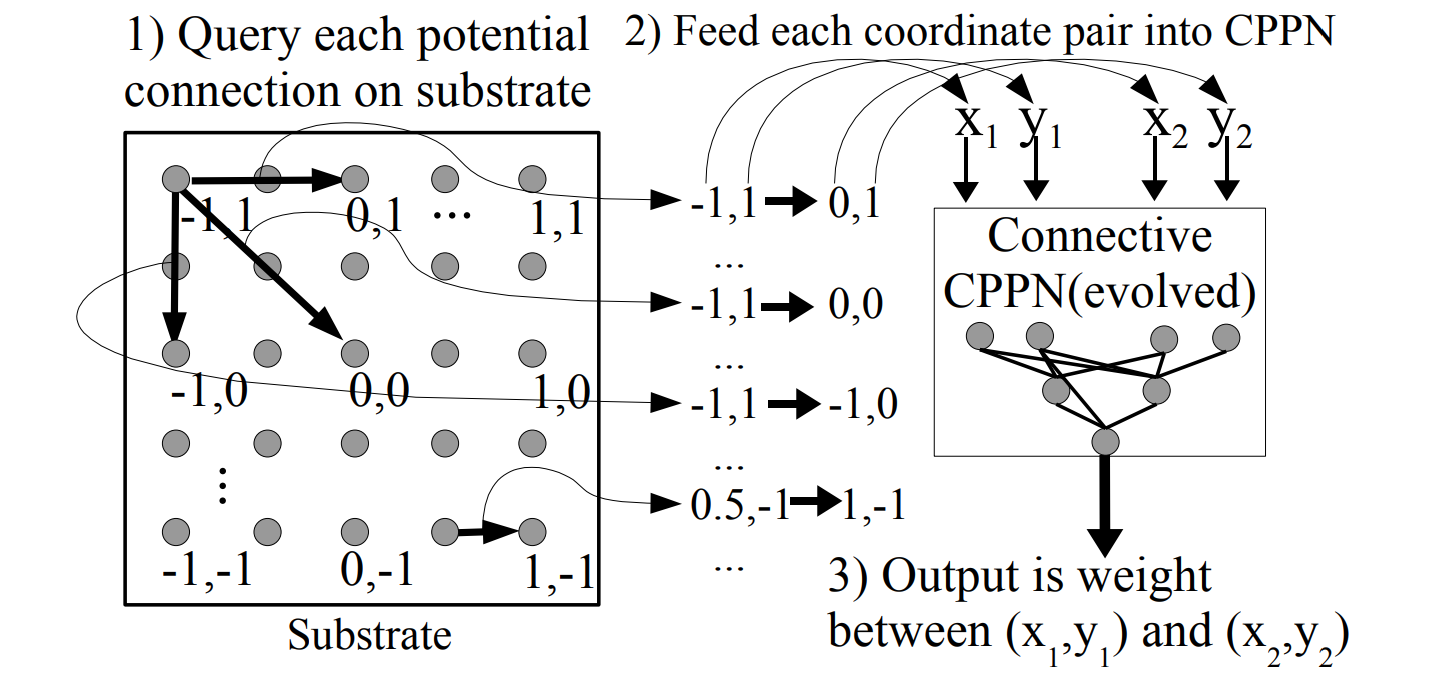
\includegraphics{images/substrat}
        }

        \caption{
            \label{substrat}
            Алгоритм получения нейронной сети из субстрата с помощью CPPN.}
    \end {center}
\end {figure}


{\parindent0pt Плюсы метода HyperNEAT:}
\begin{enumerate}[--]
    \item Наличие актуальных библиотек с реализацией на разных языках программирования: C\#, C++, Python и другие.
    \item Подходит для трудно формализируемых задач, где функция потерь и функция приспособленности могут быть не определены.
    \item Способен работать с очень большими нейронными сетями.
\end{enumerate}
%
Минусы метода HyperNEAT:
\begin{enumerate}[--]
    \item Для работы алгоритма пользователю требуется выбрать субстрат, определяющий множество возможных топологий нейронных сетей. 
    \item Намного медленнее, чем NEAT, поскольку требуется больше шагов для создания нейронных сетей на каждом из поколений.
\end{enumerate}


\subsection{Вывод}
Проанализировав плюсы и минусы обоих алгоритмов, было решено использовать NEAT, так как:

\begin{enumerate}[label=\textbullet]
    \item Нет необходимости в работе с большими нейронными сетями, поскольку оружие представляется простыми сетями, у которых только 3 ввода и 5 выводов.
    \item NEAT не использует субстрат, что позволяет генерировать сети произвольной топологии.
\end{enumerate}










%! suppress = LineBreak
\section{Разработка системы генерации оружия}

Исходный код доступен в репозитории\cite{s7}.

\subsection{Цвет и траектория снарядов}

В этом параграфе описан упрощенный алгоритм управления снарядами нейронной сетью, который может отличаться от того, что представлено в исходном коде. Этот алгоритм выполняется каждый кадр игры.

\lstset{
    emph={InverseTransformPoint, TransformDirection, AddForce, ResetState, Activate, SqrMagnitude, Sqrt, Lerp, Abs, HSVToRGB},
    emphstyle=\color{mauve},
    emph={[2]Mathf, math, Vector2, Color, neatGenomeParams},
    emphstyle={[2]\color{dkgreen}}}

\begin{lstlisting}[name=Projectile, caption={Projectile. Part 1}]
Box.ResetState(); 

Vector2 RelativePos = transform.localPosition;
float DistanceFromOrigin = RelativePos.magnitude;
float maxDistance = NNControlDistance * math.SQRT2;

_inputArr[0] = Mathf.Lerp(-1f, 1f, Mathf.Abs(RelativePos.x) / NNControlDistance);
_inputArr[1] = Mathf.Lerp(-1f, 1f, Mathf.Abs(RelativePos.y) / NNControlDistance);
_inputArr[2] = Mathf.Lerp(-1f, 1f, DistanceFromOrigin / maxDistance);
            
Box.Activate();

\end{lstlisting}

Рассмотрим подробнее этот фрагмент кода. \lstinline{_inputArr[]} -- это массив, через который нейронная сеть получает данные. Все значения, принимаемые нейронной сетью должны лежать в отрезке $[-1,1]$. Для нормализации входных данных используется встроенный в Unity метод для линейной интерполяции \lstinline{Lerp()}, а также параметр \lstinline{NNControlDistance}, подбираемый пользователем.

Чтобы у пользователя была возможность менять направление полета снарядов относительно оси у на противоположное, их паттерн должен быть симметричен относительно этой оси. Также для более приятного визуального эффекта было решено сделать паттерн симметричным и относительно оси х. Для этого в сеть подаётся модуль первых двух параметров, отвечающих за координаты.

Если обобщить, то в коде выше берутся актуальные для данного кадра позиция снаряда \lstinline{RelativePos}, его расстояние от источника \lstinline{DistanceFromOrigin} и подаются на вход в нейронную сеть после нормализации. Затем происходит активация сети \lstinline{Box.Activate()}.



\pagebreak

\begin{lstlisting}[name=Projectile, caption={Projectile. Part 2}]
float x = Mathf.Lerp(-1f, 1f, (float)_outputArr[0]) * SignX;
float y = Mathf.Lerp(-1f, 1f, (float)_outputArr[1]) * SignY;    
Vector2 forceDir = OriginTransform.TransformDirection(x, y, 0f).normalized;
    
float hue, maxSpeed, force;
hue = Mathf.Lerp(HueRange.x, HueRange.y, (float)_outputArr[2]);
maxSpeed = Mathf.Lerp(SpeedRange.x, SpeedRange.y, (float)_outputArr[3]);
force = Mathf.Lerp(ForceRange.x, ForceRange.y, (float)_outputArr[4]);

SpriteRenderer.color = Color.HSVToRGB(hue, Saturation, Brightness);
Rigidbody.AddForce(forceDir * force);

float speed = Rigidbody.velocity.magnitude;
if (speed > maxSpeed)
    Rigidbody.velocity = Rigidbody.velocity.normalized * maxSpeed;

transform.up = Rigidbody.velocity;
\end{lstlisting}

После активации сети можно считывать выходные данные через массив \lstinline{_outputArr[]}. Сеть выдает все значения в отрезке $[0,1]$. Данные с первых двух выходов \lstinline{_outputArr[0]} и \lstinline{_outputArr[1]}, отвечающих за $x$ и $y$ компоненты скорости, сначала преобразуются в отрезки $[-1,1]$. Затем на их основе строится нормированный вектор силы \lstinline{forceDir}, который потом прилагается к снаряду посредством метода \lstinline{AddForce}.

Так было сделано для плавности и реалистичности полета снарядов, если бы нейронная сеть меняла их скорость напрямую, они бы двигались дёрганно и слишком резко. Чтобы под действием силы скорость снаряда не росла до бесконечности, она ограничена параметром \lstinline{maxSpeed}.

Изначально планировалось использовать цветовую модель RGB, но возникли проблемы с контролем цветов, которые может выдавать сеть. Например, если у игры темный фон, то снаряды должны быть ярких оттенков, чтобы не сливаться с ним. У пользователя должна быть возможность задать желаемое пространство цветов, внутри которого будут заключены значения нейронной сети. RGB представляет цвета в виде точек в трехмерном пространстве, поэтому выделить такое пространство было бы затруднительно.

Эту проблему решает цветовая модель HSV (Hue, Saturation, Value — тон, насыщенность, значение), в которой цвет представляется более интуитивно понятным образом. Компонента \lstinline{hue} задается в виде отрезка, минимальное и максимальное значение которого выбирается пользователем. \lstinline{Saturation} и \lstinline{Value} задаются как константы и тоже могут быть изменены пользователем.



\subsection{Параметры оружия}
Для точной настройки оружия было добавлено 29 параметров, которые контролируются пользователем.

\vspace{5mm}

\textbf{Параметры стрельбы.} Эти параметры регулируют скорострельность и начальную фазу полета снарядов:
\begin{enumerate}
    \item {\small \textbf{FireRate}} -- Время в секундах между каждой очередью или выстрелом.
    \item {\small \textbf{ProjectilesInOneShot}} -- Количество снарядов в очереди или выстреле.
    \item {\small \textbf{WeaponMode}} -- Определяет режим стрельбы. Их два:
    \begin{enumerate}[label=\textbullet]
        \item {\small \textbf{MultiShot}} -- Одиночный выстрел, состоящий из множества снарядов. Снаряды вылетают полукругом, который определяется параметром {\small \textbf{Angle}}.
        \item {\small \textbf{Burst}} -- Очередь, при которой снаряды вылетают по одному.
    \end{enumerate}
    \item {\small \textbf{BurstMode}} -- Определяет подвид стрельбы очередью. Их шесть:
    \begin{enumerate}[label=\textbullet]
        \item {\small \textbf{Clockwise}} -- Снаряды вылетают полукругом. Первый с максимальным углом, последний с минимальным. {\small \textbf{SignX}} у первой половины положительный, у второй -- отрицательный.
        \item {\small \textbf{CounterClockwise}} -- Снаряды вылетают полукругом. Первый с минимальным углом, последний с максимальным. {\small \textbf{SignX}} у первой половины отрицательный, у второй -- положительный.
        \item {\small \textbf{Alternate}} -- Начальные траектории снарядов чередуются от большего угла к меньшему. {\small \textbf{SignX}} чередует знак.
        \item {\small \textbf{Straight}} -- Снаряды летят прямо. {\small \textbf{SignX}} чередуется знак.
        \item {\small \textbf{MaxMinAngle}} -- Одна половина снарядов летит с максимальным углом, другая -- с минимальным.
        \item {\small \textbf{Random}} -- Угол и знак {\small \textbf{SignX}} выбираются случайно.
    \end{enumerate}
    \item {\small \textbf{BurstRate}} -- Время в секундах между снарядами при стрельбе очередью.
\end{enumerate}

\vspace{5mm}

\textbf{Параметры систем координат.} Системы координат являются родителями снарядов в иерархии сцены, поэтому при их движении движутся и снаряды. Регулируя эти параметры, можно создавать более сложное оружие:
\begin{enumerate}
    \setcounter{enumi}{5}
    \item {\small \textbf{RotationSpeed}} -- Вращение систем координат в градусах в секунду при нажатии кнопки запуска. Если значение отрицательное, вращение будет в противоположном направлении.
    \item {\small \textbf{MoveSpeed}} -- Скорость систем координат при нажатии кнопки запуска.
\end{enumerate}

\vspace{5mm}

\textbf{Параметры снарядов.} Эти параметры отвечают за поведение и внешний вид снарядов:
\begin{enumerate}
    \setcounter{enumi}{7}
    \item {\small \textbf{NetworkControlMode}} -- Определяет, как сеть управляет снарядом. Есть два режима:
    \begin{enumerate}[label=\textbullet]
        \item {\small \textbf{ForceSum}} -- Сеть выдает вектор силы, который затем суммируется с вектором силы, уже действующим на снаряд.
        \item {\small \textbf{VelocitySum}} -- Сеть выдает вектор скорости, который затем суммируется с вектором скорости, которым уже обладает снаряд.
    \end{enumerate}
    \item {\small \textbf{ReadMode}} -- Определяет, каким образом из выходных параметров $(x, y)$ формируется вектор $\overrightarrow{dir}$, определяющий направление скорости или силы. Есть два режима:
    \begin{enumerate}[label=\textbullet]
        \item {\small \textbf{Default}}: \[ \overrightarrow{dir}=x\hat{x}+y\hat{y}, \]
        где $\hat{x}, \hat{y}$ -- орты локальной системы координат снаряда с началом в точке выстрела.

        \item {\small \textbf{Rotator}}: \[ \overrightarrow{dir}=x\hat{q}+y\hat{r}, \]
        где $\hat{r}$ -- орт радиус-вектора снаряда, и $\hat{q} \perp \hat{r}$.

    \end{enumerate}
    \item {\small \textbf{Size}} -- Размер снаряда. Для рендеринга снарядов используется текстура круга. Изменяя этот параметр, можно получать снаряды в форме эллипсов.
    \item {\small \textbf{Lifespan}} -- Срок жизни снаряда в секундах. По истечению этого срока снаряд уничтожается.
    \item {\small \textbf{HueRange}} -- Диапазон возможных значений для цветовой компоненты hue. Точное значение зависит от вывода нейронной сети.
    \item {\small \textbf{Saturation}} -- Цветовая компонента Saturation.
    \item {\small \textbf{Brightness}} -- Цветовая компонента Value.
\end{enumerate}

\vspace{5mm}

\textbf{Параметры паттерна.} Эти параметры определяют настройки, связанные входными и выходными значениями нейронной сети:
\begin{enumerate}
    \setcounter{enumi}{14}
    \item {\small \textbf{SpeedRange}} -- Диапазон возможных значений для максимальной скорости снаряда. Точное значение зависит от вывода нейронной сети.
    \item {\small \textbf{ForceRange}} -- Диапазон возможных значений силы, приложенной к снаряду. Точное значение зависит от вывода нейронной сети.
    \item {\small \textbf{NNControlDistance}} -- Определяет область, в которой снаряды управляются нейронной сетью.
    \item {\small \textbf{SignX}} -- Множитель вывода х. Если он равен нулю, вывод будет проигнорирован.
    \item {\small \textbf{SignY}} -- Множитель вывода у. Если он равен нулю, вывод будет проигнорирован.
    \item {\small \textbf{ForwardForce}} -- Прилагать ли к снаряду силу, направленную вперед. Эта сила равна выводу force нейронной сети.
\end{enumerate}

\vspace{5mm}

\textbf{Параметры начальной фазы:}
\begin{enumerate}
    \setcounter{enumi}{20}
    \item {\small \textbf{InitialFlightRadius}} -- Определяет область, в которой снаряды находятся в состоянии начальной фазы. В этом состоянии снаряды не управляются нейронной сетью, вместо этого они движутся с постоянной начальной скоростью.
    \item {\small \textbf{InitialSpeed}} -- Длина вектора начальной скорости.
    \item {\small \textbf{Angle}} -- Максимальный угол между начальной скоростью снаряда и вертикальной осью игрового объекта оружия.
\end{enumerate}

\vspace{5mm}

\textbf{Параметры отражения:}
\begin{enumerate}
    \setcounter{enumi}{23}
    \item {\small \textbf{FlipXOnReflect}} -- Изменять ли значение {\small \textbf{SignX}} на противоположное после отражения.
    \item {\small \textbf{FlipYOnReflect}} -- Изменять ли значение {\small \textbf{SignY}} на противоположное после отражения.
    \item {\small \textbf{Mode}} -- Определяет границы, от которых снаряд отражается. Есть три режима:
    \begin{enumerate}[label=\textbullet]
        \item {\small \textbf{CircleReflection}} -- Границей является окружность.
        \item {\small \textbf{RectangleReflection}} -- Границей является прямоугольник.
        \item {\small \textbf{Polar}} -- Границей является угол.
    \end{enumerate}
    \item {\small \textbf{ReflectiveCircleRadius}} -- Радиус границы-окружности.
    \item {\small \textbf{RectDimensions}} -- Размеры границы-прямоугольника.
    \item {\small \textbf{MaxPolarAngleDeg}} -- Максимально возможный полярный угол.
\end{enumerate}

\pagebreak


\subsection{Пользовательский интерфейс}

Для создания кастомных окон инспектора использовалась система\\ IMGUI\cite{s10}, которая предназначена для расширения функциональности Unity и разработки инструментов для разработчиков.

\begin{figure}[ht]
    \begin{center}
        \scalebox{0.4}{
            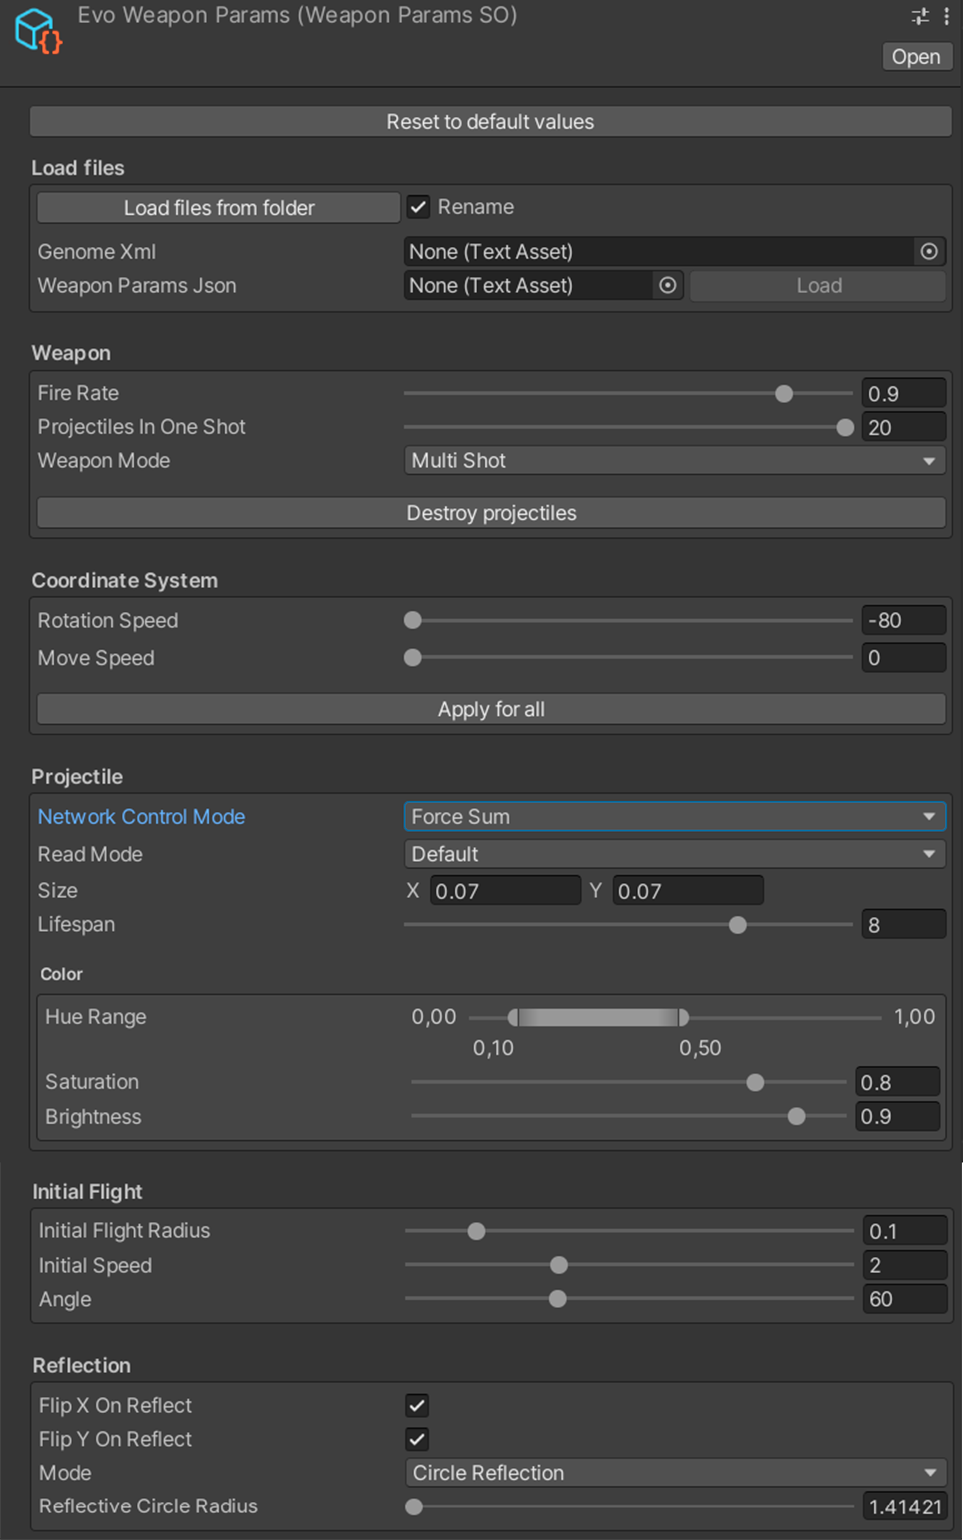
\includegraphics{images/Inspector}
        }

        \caption{
            \label{Inspector}
            Кастомный инспектор параметров оружия.}
    \end {center}
\end {figure}

Особенности инспектора параметров оружия:
\begin{enumerate}[label=\textbullet]
    \item Кнопка {\small \textbf{Reset to default values}}, возвращающая параметры к начальным значениям, заданным разработчиком.
    \item Раздел {\small \textbf{Load files}} для загрузки генома и параметров с файлов.
    \item Кнопка {\small \textbf{Destroy Projectiles}}, уничтожающая снаряды.
    \item Двойные слайдеры, позволяющие задавать два значения: минимальное и максимальное.
    \item Интерфейс подстраивается под выбранные значения. К примеру, если в параметре {\small \textbf{Weapon Mode}} будет выбран режим {\small \textbf{Burst}}, появятся поля {\small \textbf{Burst Mode}} и {\small \textbf{Burst Rate}}.
    \item Есть поддержка редактирования нескольких объектов.
    \item Есть поддержка истории редактирования. То есть Undo/Redo.
\end{enumerate}

\begin{figure}[ht]
    \begin{center}
        \scalebox{0.6}{
            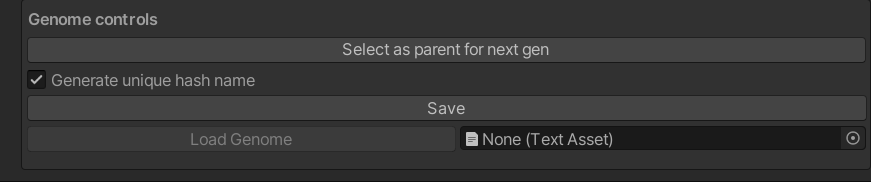
\includegraphics{images/savingWeapons}
        }

        \caption{
            \label{SavingWeapon}
            Кастомный инспектор оружия.}
    \end {center}
\end {figure}

Особенности инспектора оружия:
\begin{enumerate}[label=\textbullet]
    \item Кнопка {\small \textbf{Select as parent for next gen}}, позволяющая пользователю выбирать понравившиеся геномы.
    \item Кнопка {\small \textbf{Save}} для сохранения генома и параметров оружия.
    \item Флажок {\small \textbf{Generate unique hash name}}. Если отмечен, то при сохранении названия файлов генерируется автоматически.
    \item Есть поддержка редактирования нескольких объектов.
\end{enumerate}


\subsection{Система эволюции оружия}

\textbf{Выбор библиотеки.} Для эволюции нейронных сетей была выбрана библиотека SharpNEAT\cite{s8} версии 2.4.4, реализующая алгоритм NEAT на языке C\#. Выбор этой библиотеки и её версии обусловлен в первую очередь совместимостью с игровым движком Unity.

Существует SharpNEAT версии 4.0.0, в которой значительно улучшена производительность и удобство программного интерфейса, но целевая платформа этой версии -- .NET Core, несовместимая с Unity. По этой причине выбор остановился на более ранней версии 2.4.4.

Для использования библиотеки в Unity необходимо создать её DLL в какой-либо среде разработки и поместить эту DLL в специальную папку \flqq Plugins\frqq. Плагины в Unity могут быть на трех языках: C, C++, C\#. Плагины на C\# доступны в бесплатной версии Unity, а вот для использования плагинов на других двух языках придется покупать профессиональную версию.




\textbf{Параметры алгоритма NEAT.} Обычно NEAT используют для эволюции огромного количества нейронных сетей на протяжении множества поколений с помощью функции приспособленности, заданной математически. В нашем случае функцией приспособленности является человек -- игрок или разработчик игры, поскольку задача оценки эстетичности и полезности паттернов не является строго формализируемой. По этой причине оцениваемая популяция и количество поколений не должны быть большими.

Приведенные ниже значения параметров были получены опытным путем, остальные параметры сохранили значение по умолчанию. Параметры подбирались таким образом, чтобы интересные паттерны в среднем выводились за 10-15 поколений.

\begin{lstlisting}[caption={Params}]
PopulationSize = 6;
CloneOffspringCount = 2;
SexualOffspringCount = 4;
neatGenomeParams.InitialInterconnectionsProportion = 0.2;
neatGenomeParams.AddConnectionMutationProbability = 0.7;
neatGenomeParams.AddNodeMutationProbability = 0.7;
neatGenomeParams.ConnectionWeightMutationProbability = 0.8;
neatGenomeParams.DisjointExcessGenesRecombinedProbability = 0.5;
neatGenomeParams.NodeAuxStateMutationProbability = 0.2;
\end{lstlisting}
Краткое описание этих параметров:
\begin{enumerate}[label=\textbullet]
    \item PopulationSize -- Количество геномов, подвергаемых эволюции.
    \item CloneOffspringCount -- Сколько геномов создается путем клонирования.
    \item SexualOffspringCount -- Сколько геномов создается путем полового размножения.
    \item InitialInterconnectionsProportion -- Плотность нейронных сетей первого поколения.
    \item AddConnectionMutationProbability -- Вероятность появления нового ребра.
    \item AddNodeMutationProbability -- Вероятность появления нового узла.
    \item ConnectionWeightMutationProbability -- Вероятность изменения веса ребра.
    \item DisjointExcessGenesRecombinedProbability -- Вероятность копирования всех не совпавших генов в один из потомков при половом размножении.
    \item NodeAuxStateMutationProbability -- Вероятность узла приобрести дополнительное состояние (стать неактивным).
\end{enumerate}

\pagebreak

\textbf{Создание нового поколения.} Для создания нового поколения оружия необходимо выбрать родителей, на основе которых оно построится. Пользователь может выбрать любое их количество:

\begin{enumerate}[label=\textbullet]
    \item Если пользователь не выбрал ни одного генома, программа случайно выберет два.
    \item Если пользователь выбрал один геном, то этот геном будет скрещен с не выбранными.
    \item Если пользователь выбрал два или более геномов, то выбранные геномы будут скрещены между собой.
\end{enumerate}

\begin{figure}[ht]
    \begin{center}
        \scalebox{0.4}{
            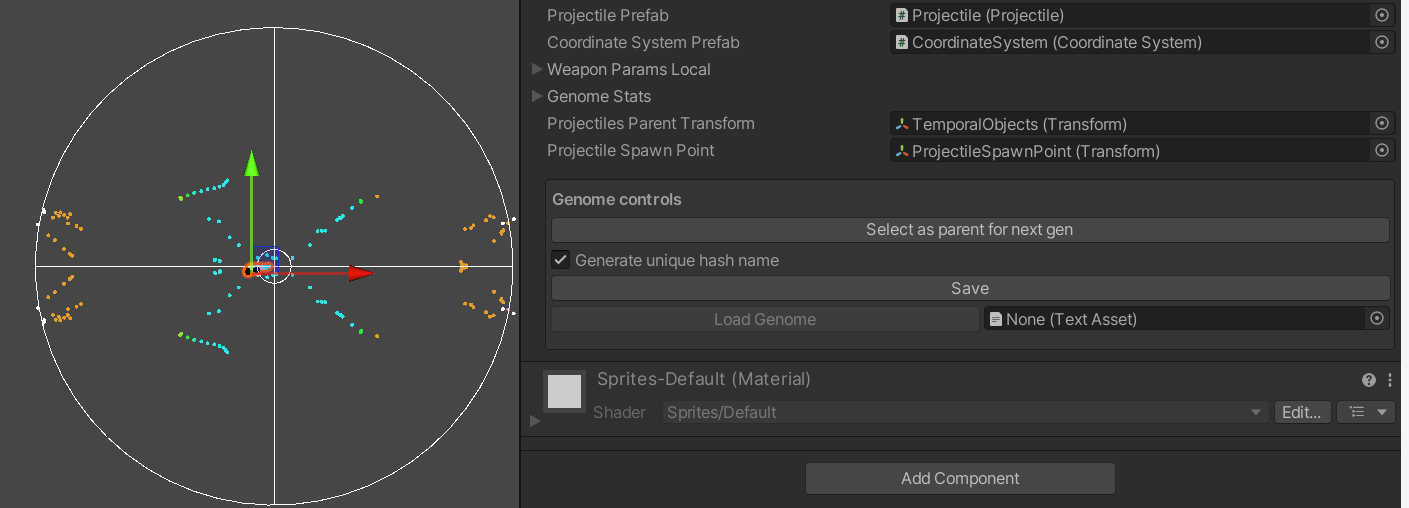
\includegraphics{images/SelectWeapon}
        }

        \caption{
            \label{SelectWeapon}
            Выбор родителей для нового поколения.}
    \end {center}
\end {figure}

Чтобы выбрать геном в качестве родителя, нужно выбрать игровой объект оружия и в его инспекторе нажать кнопку {\small \textbf{Select as parent for next gen}}. После того как нужное количество родителей было выбрано, нужно нажать на кнопку {\small \textbf{New Generation}}.

\begin{figure}[ht]
    \begin{center}
        \scalebox{0.15}{
            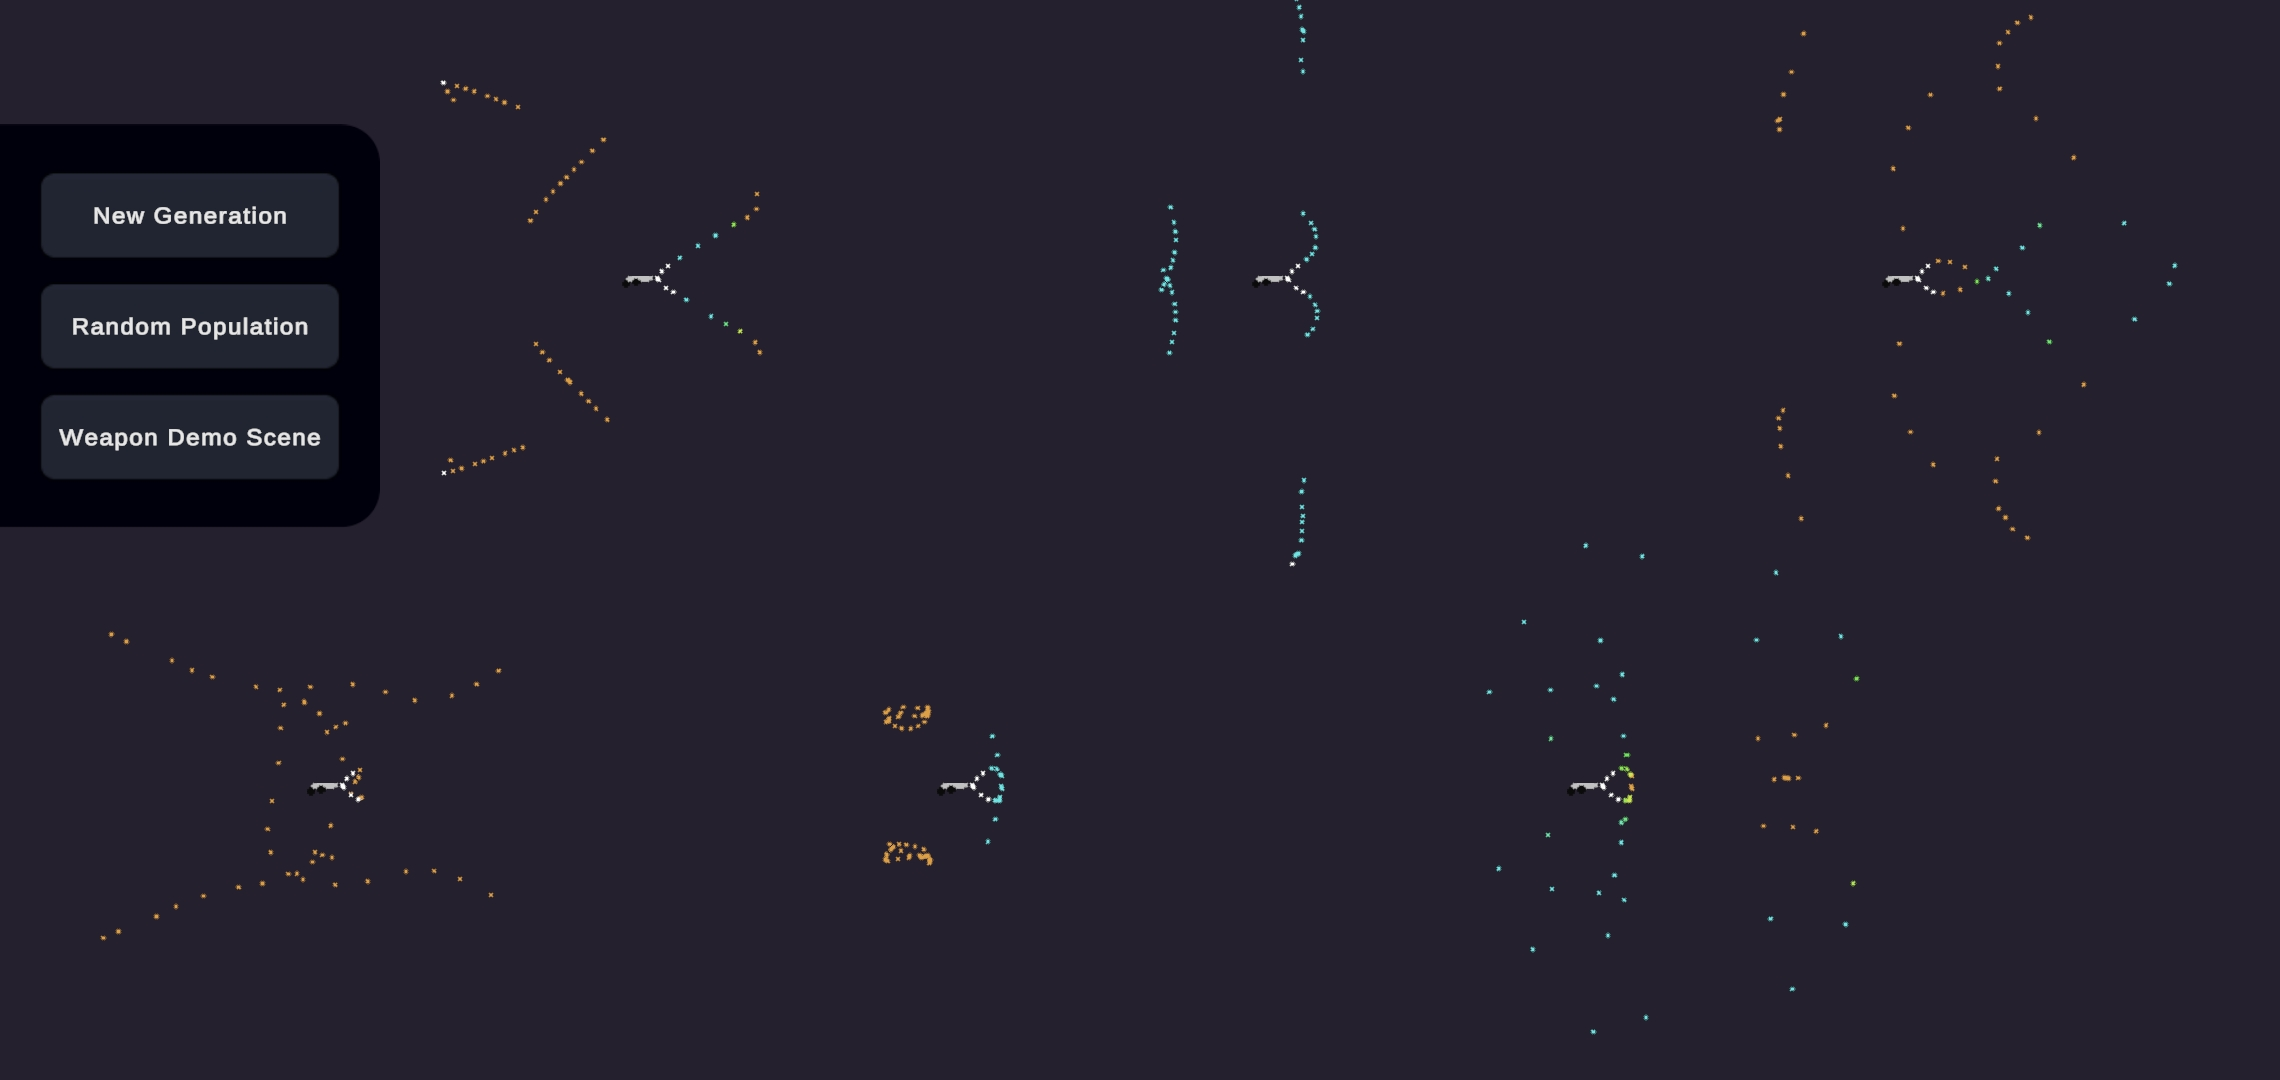
\includegraphics{images/EvoScene}
        }

        \caption{
            \label{EvoScene}
            Сцена эволюции оружия.}
    \end {center}
\end {figure}

Если эволюция зашла в тупик, нужно нажать на кнопку {\small \textbf{Random Population}}, которая создаст случайное поколение.

\subsection{Сохранение оружия}

Чтобы сохранить понравившееся оружие, нужно выбрать игровой объект оружия и в его инспекторе (Рисунок~\ref{SelectWeapon}) нажать кнопку {\small \textbf{Save.}} Будет создано и сохранено два файла:

\begin{enumerate}[label=\textbullet]
    \item {\small \textbf{Genome\_<UniqueHash>.xml}} содержит в себе информацию об узлах нейронной сети и функциях активации.
    \item {\small \textbf{Params\_<UniqueHash>.json}} является представлением параметров оружия в формате json.
\end{enumerate}


\section{Разработка игры}

WebGL сборку проекта можно посмотреть здесь\cite{s9}.

\subsection{Документация}
Для публикации Unity требует документацию ассета на английском. Для написания документации использовалась система генерации статических сайтов Jekyll\cite{s11} и тема Just the Docs\cite{s12}. Документация доступна здесь\cite{s13}.


\subsection{Демонстрационные сцены}
Для демонстрационных целей было создано три сцены:

\begin{enumerate}[label=\textbullet]
    \item \textbf{Weapon Demo} -- сцена, в которой демонстрируется 140 оружий, заранее созданных разработчиком. Кроме того, в этой сцене есть визуализация силовых полей, действующих на снаряды.

    \begin{figure}[ht]
        \begin{center}
            \scalebox{0.15}{
                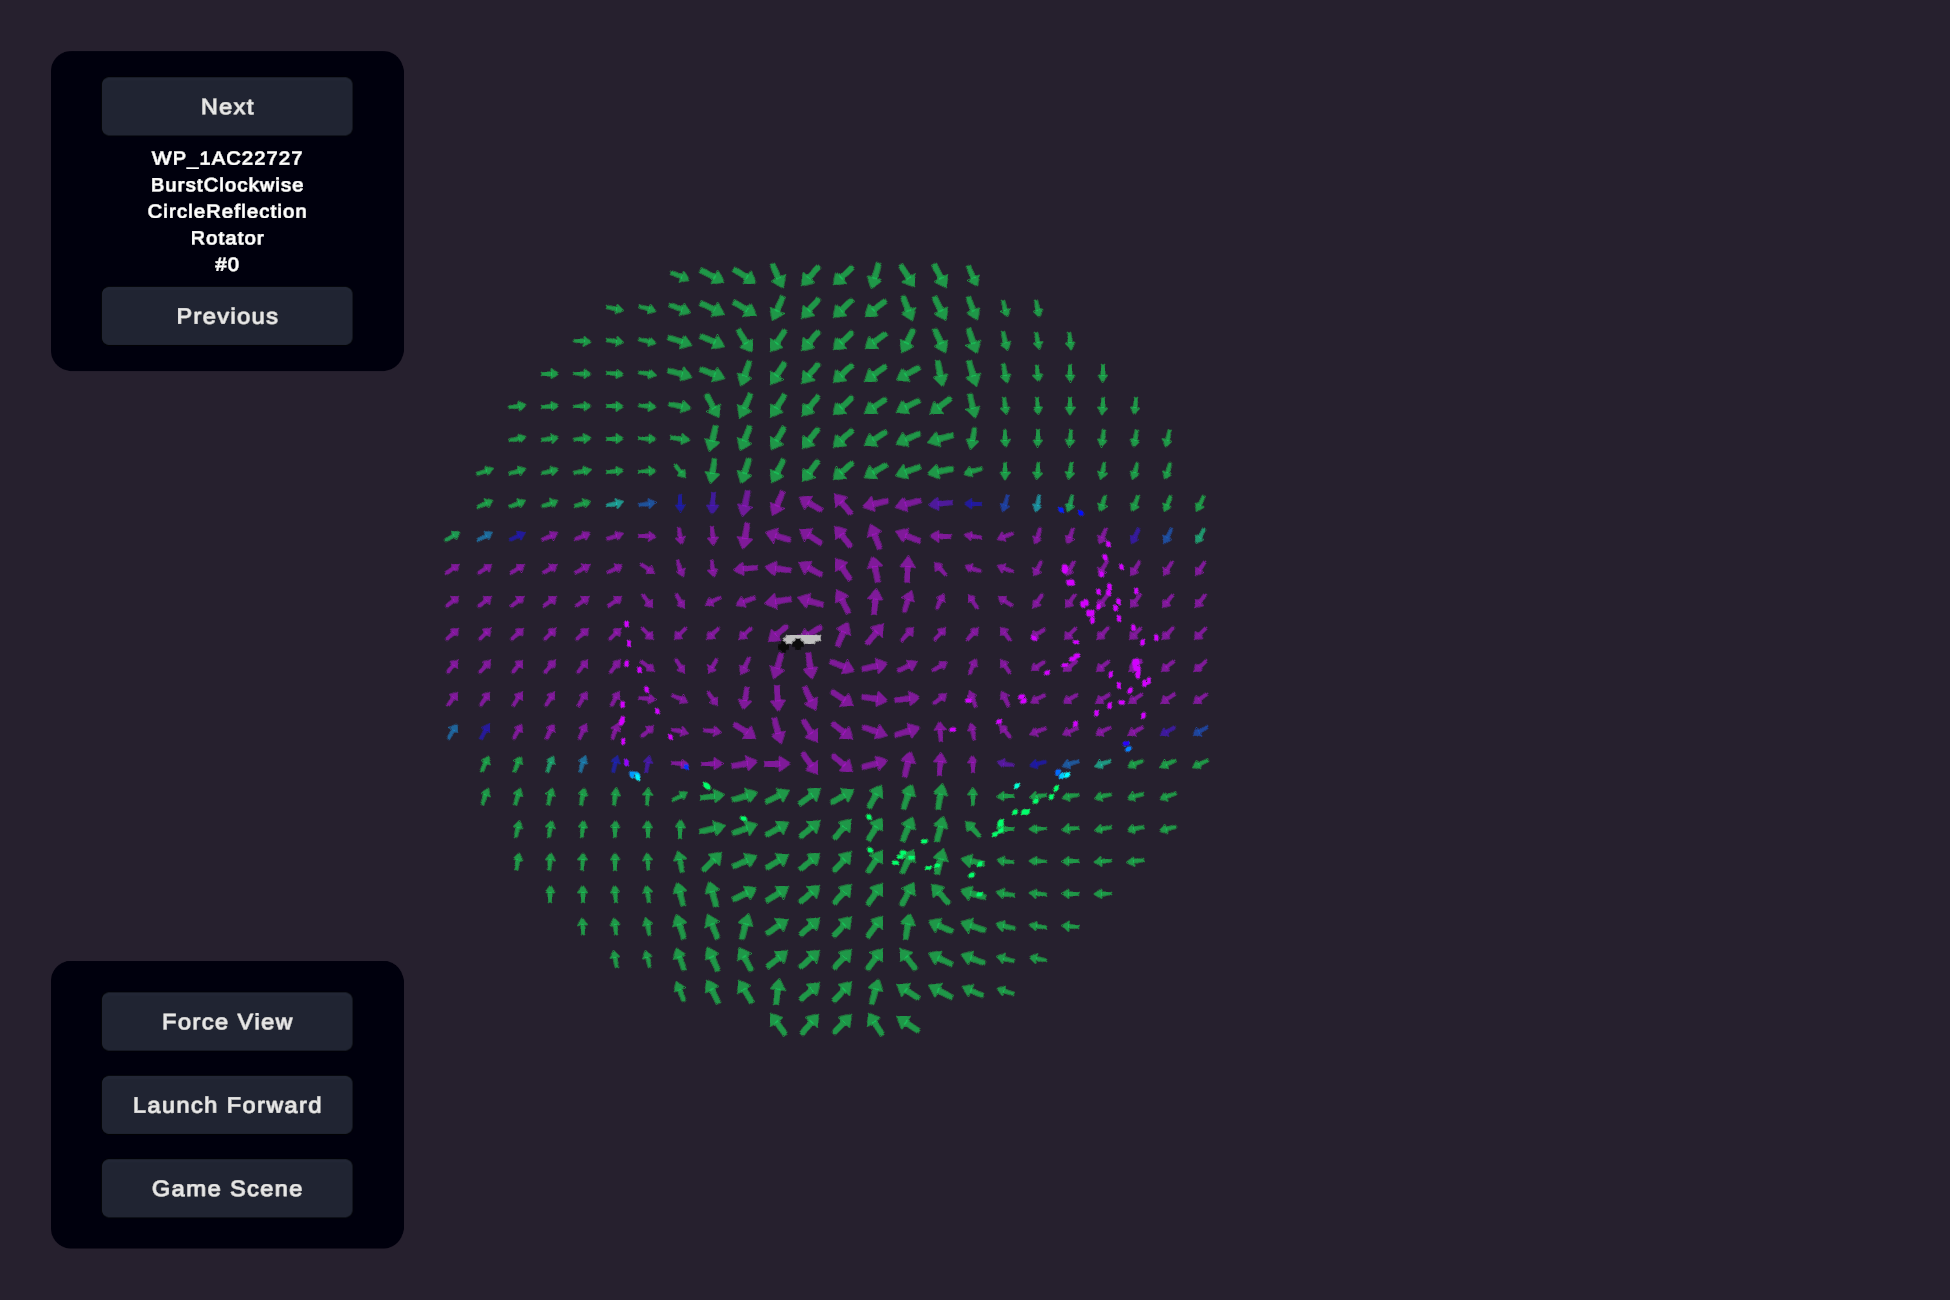
\includegraphics{images/WeaponDemo}
            }

            \caption{
                \label{WeaponDemo}
                Weapon Demo.}
        \end {center}
    \end {figure}

    \textbf{Замечание.} Разные группы снарядов могут иметь разные значения параметров {\small \textbf{SignY}} и {\small \textbf{SignX,}} поэтому визуализация силового поля может быть некорректна для каких-то из них.


    \item \textbf{Shadow Survival} -- простая игра в жанре <<Shoot ’em up>>. Во время игры генерируется оружие, которое можно подобрать и настроить некоторые параметры.

    \begin{figure}[ht]
        \begin{center}
            \scalebox{0.2}{
                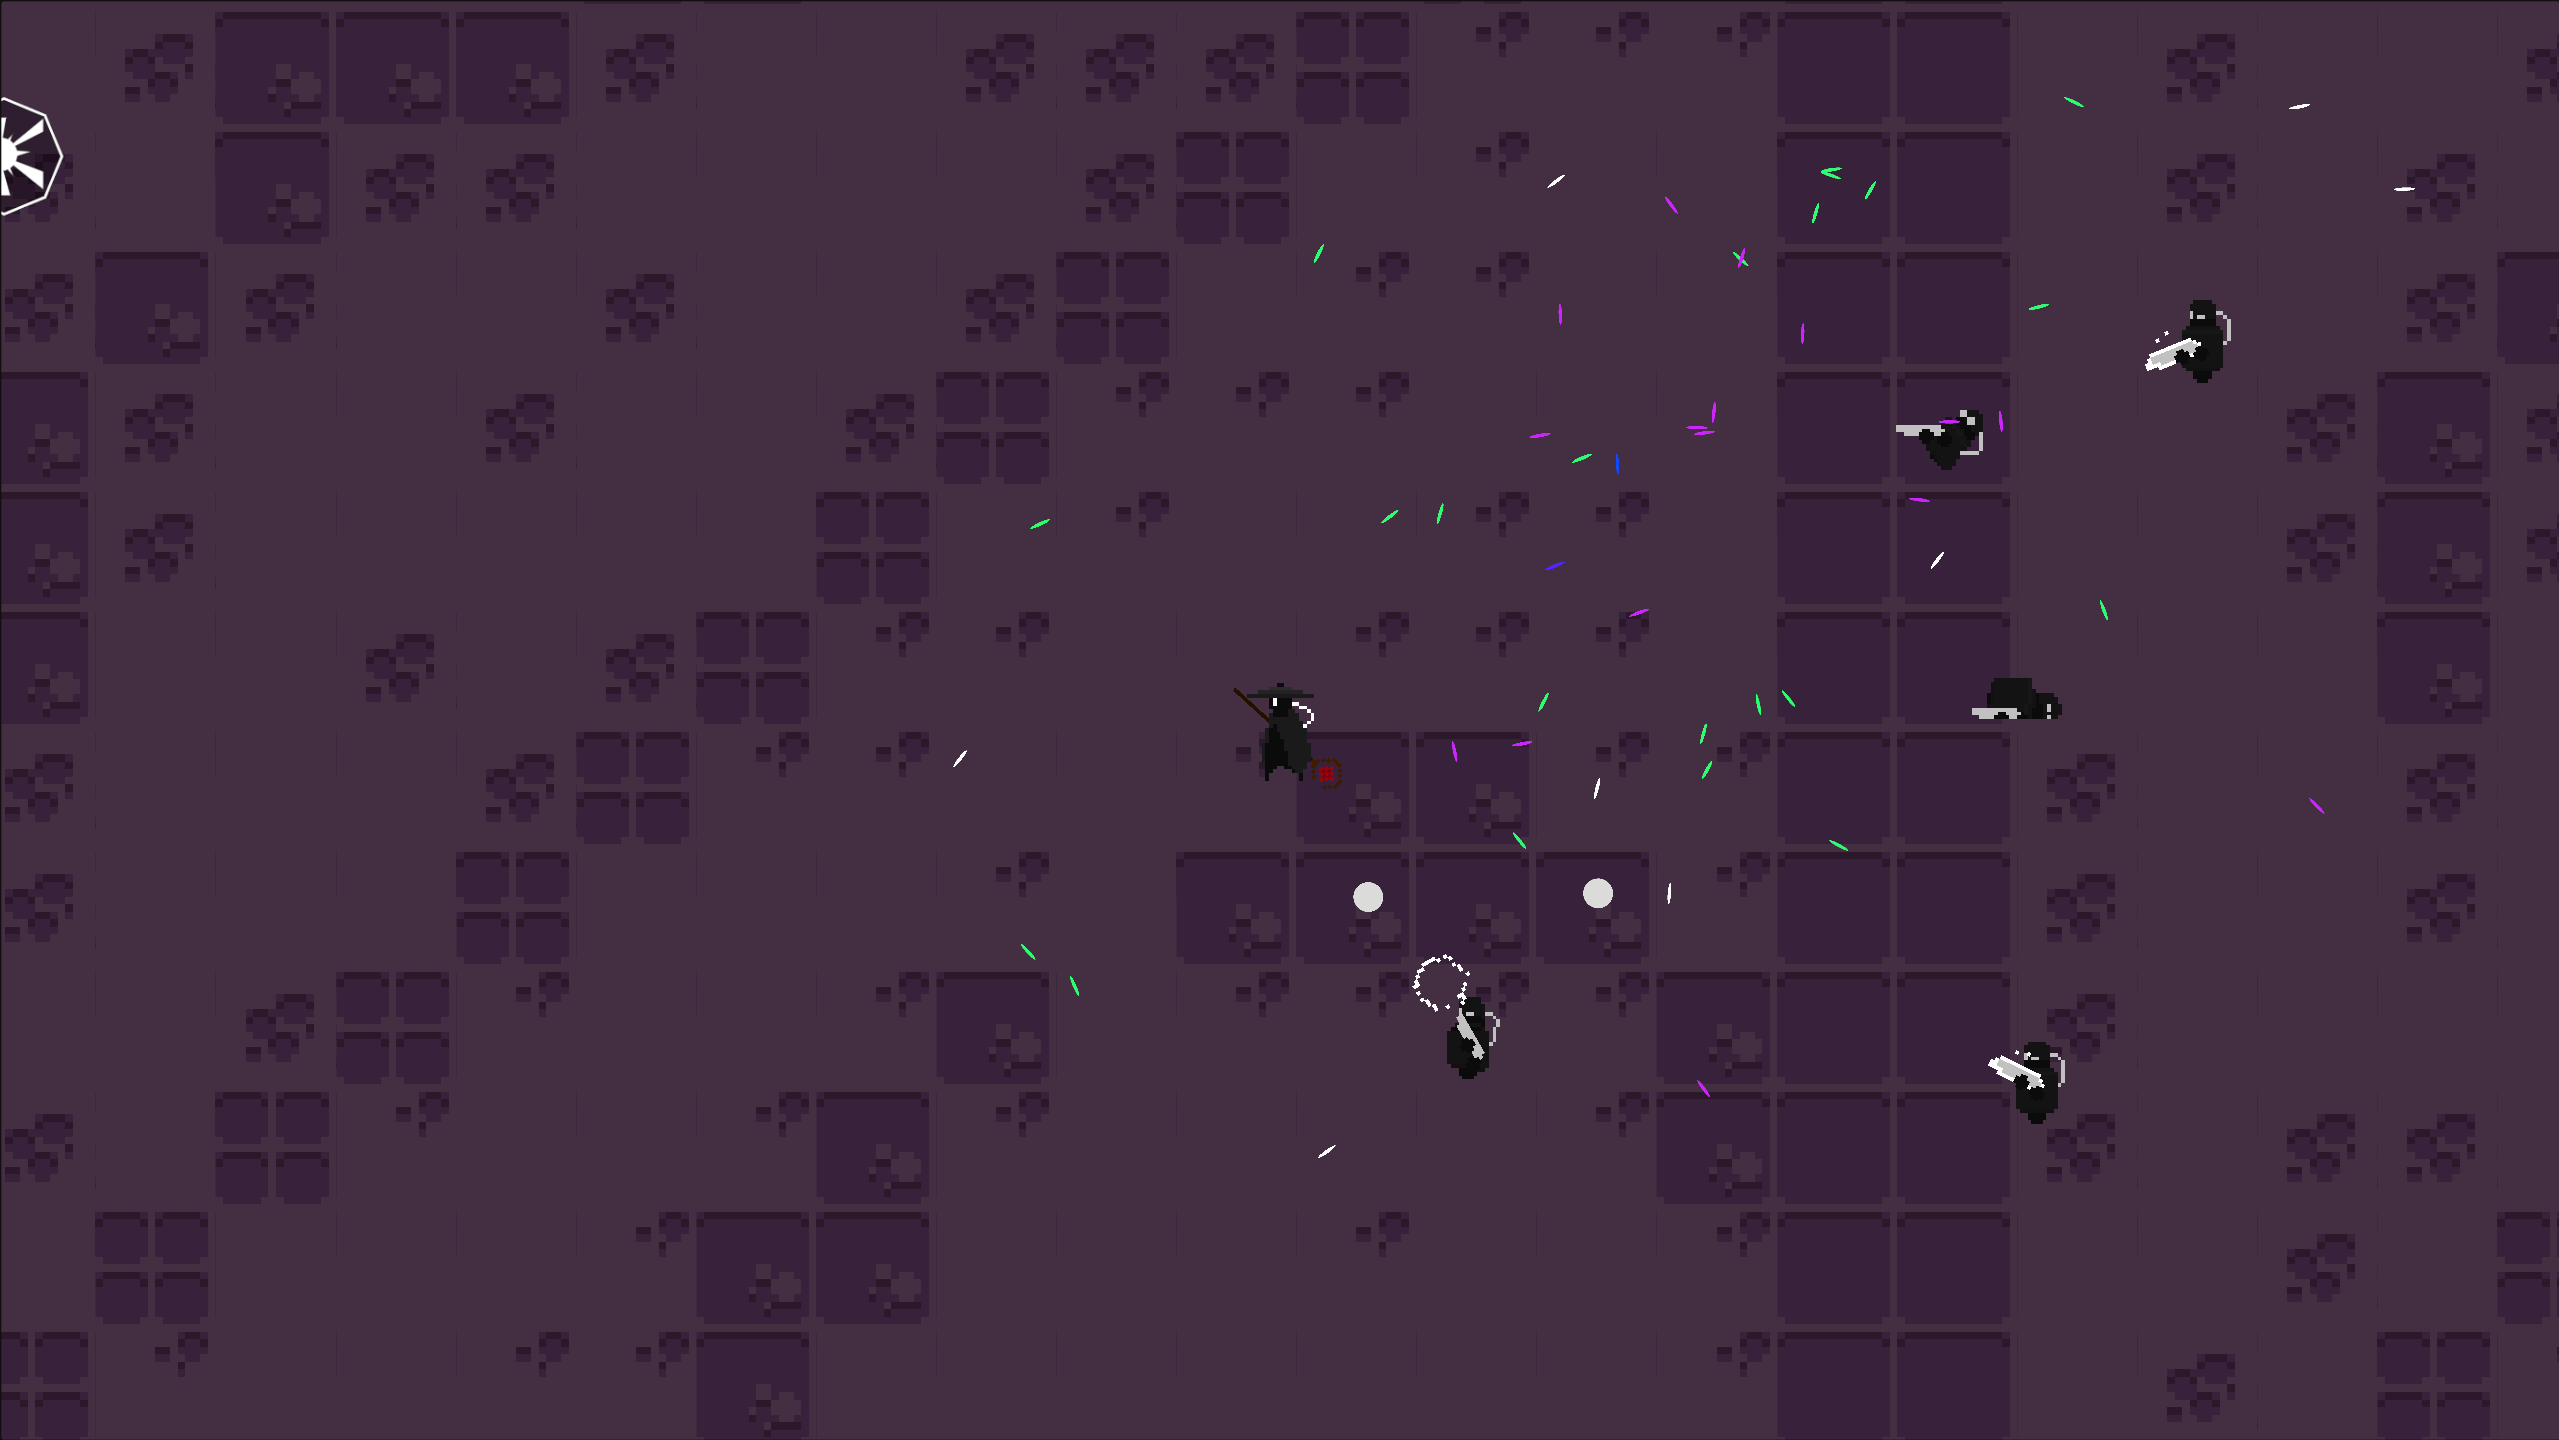
\includegraphics{images/ShadowSurvival}
            }

            \caption{
                \label{ShadowSurvival}
                Shadow Survival.
            }
        \end {center}
    \end {figure}

    \item \textbf{Space Shooter} -- простая игра тоже в жанре <<Shoot ’em up>>. Здесь оружие генерируется у врагов случайным образом.

    \begin{figure}[ht]
        \begin{center}
            \scalebox{0.2}{
                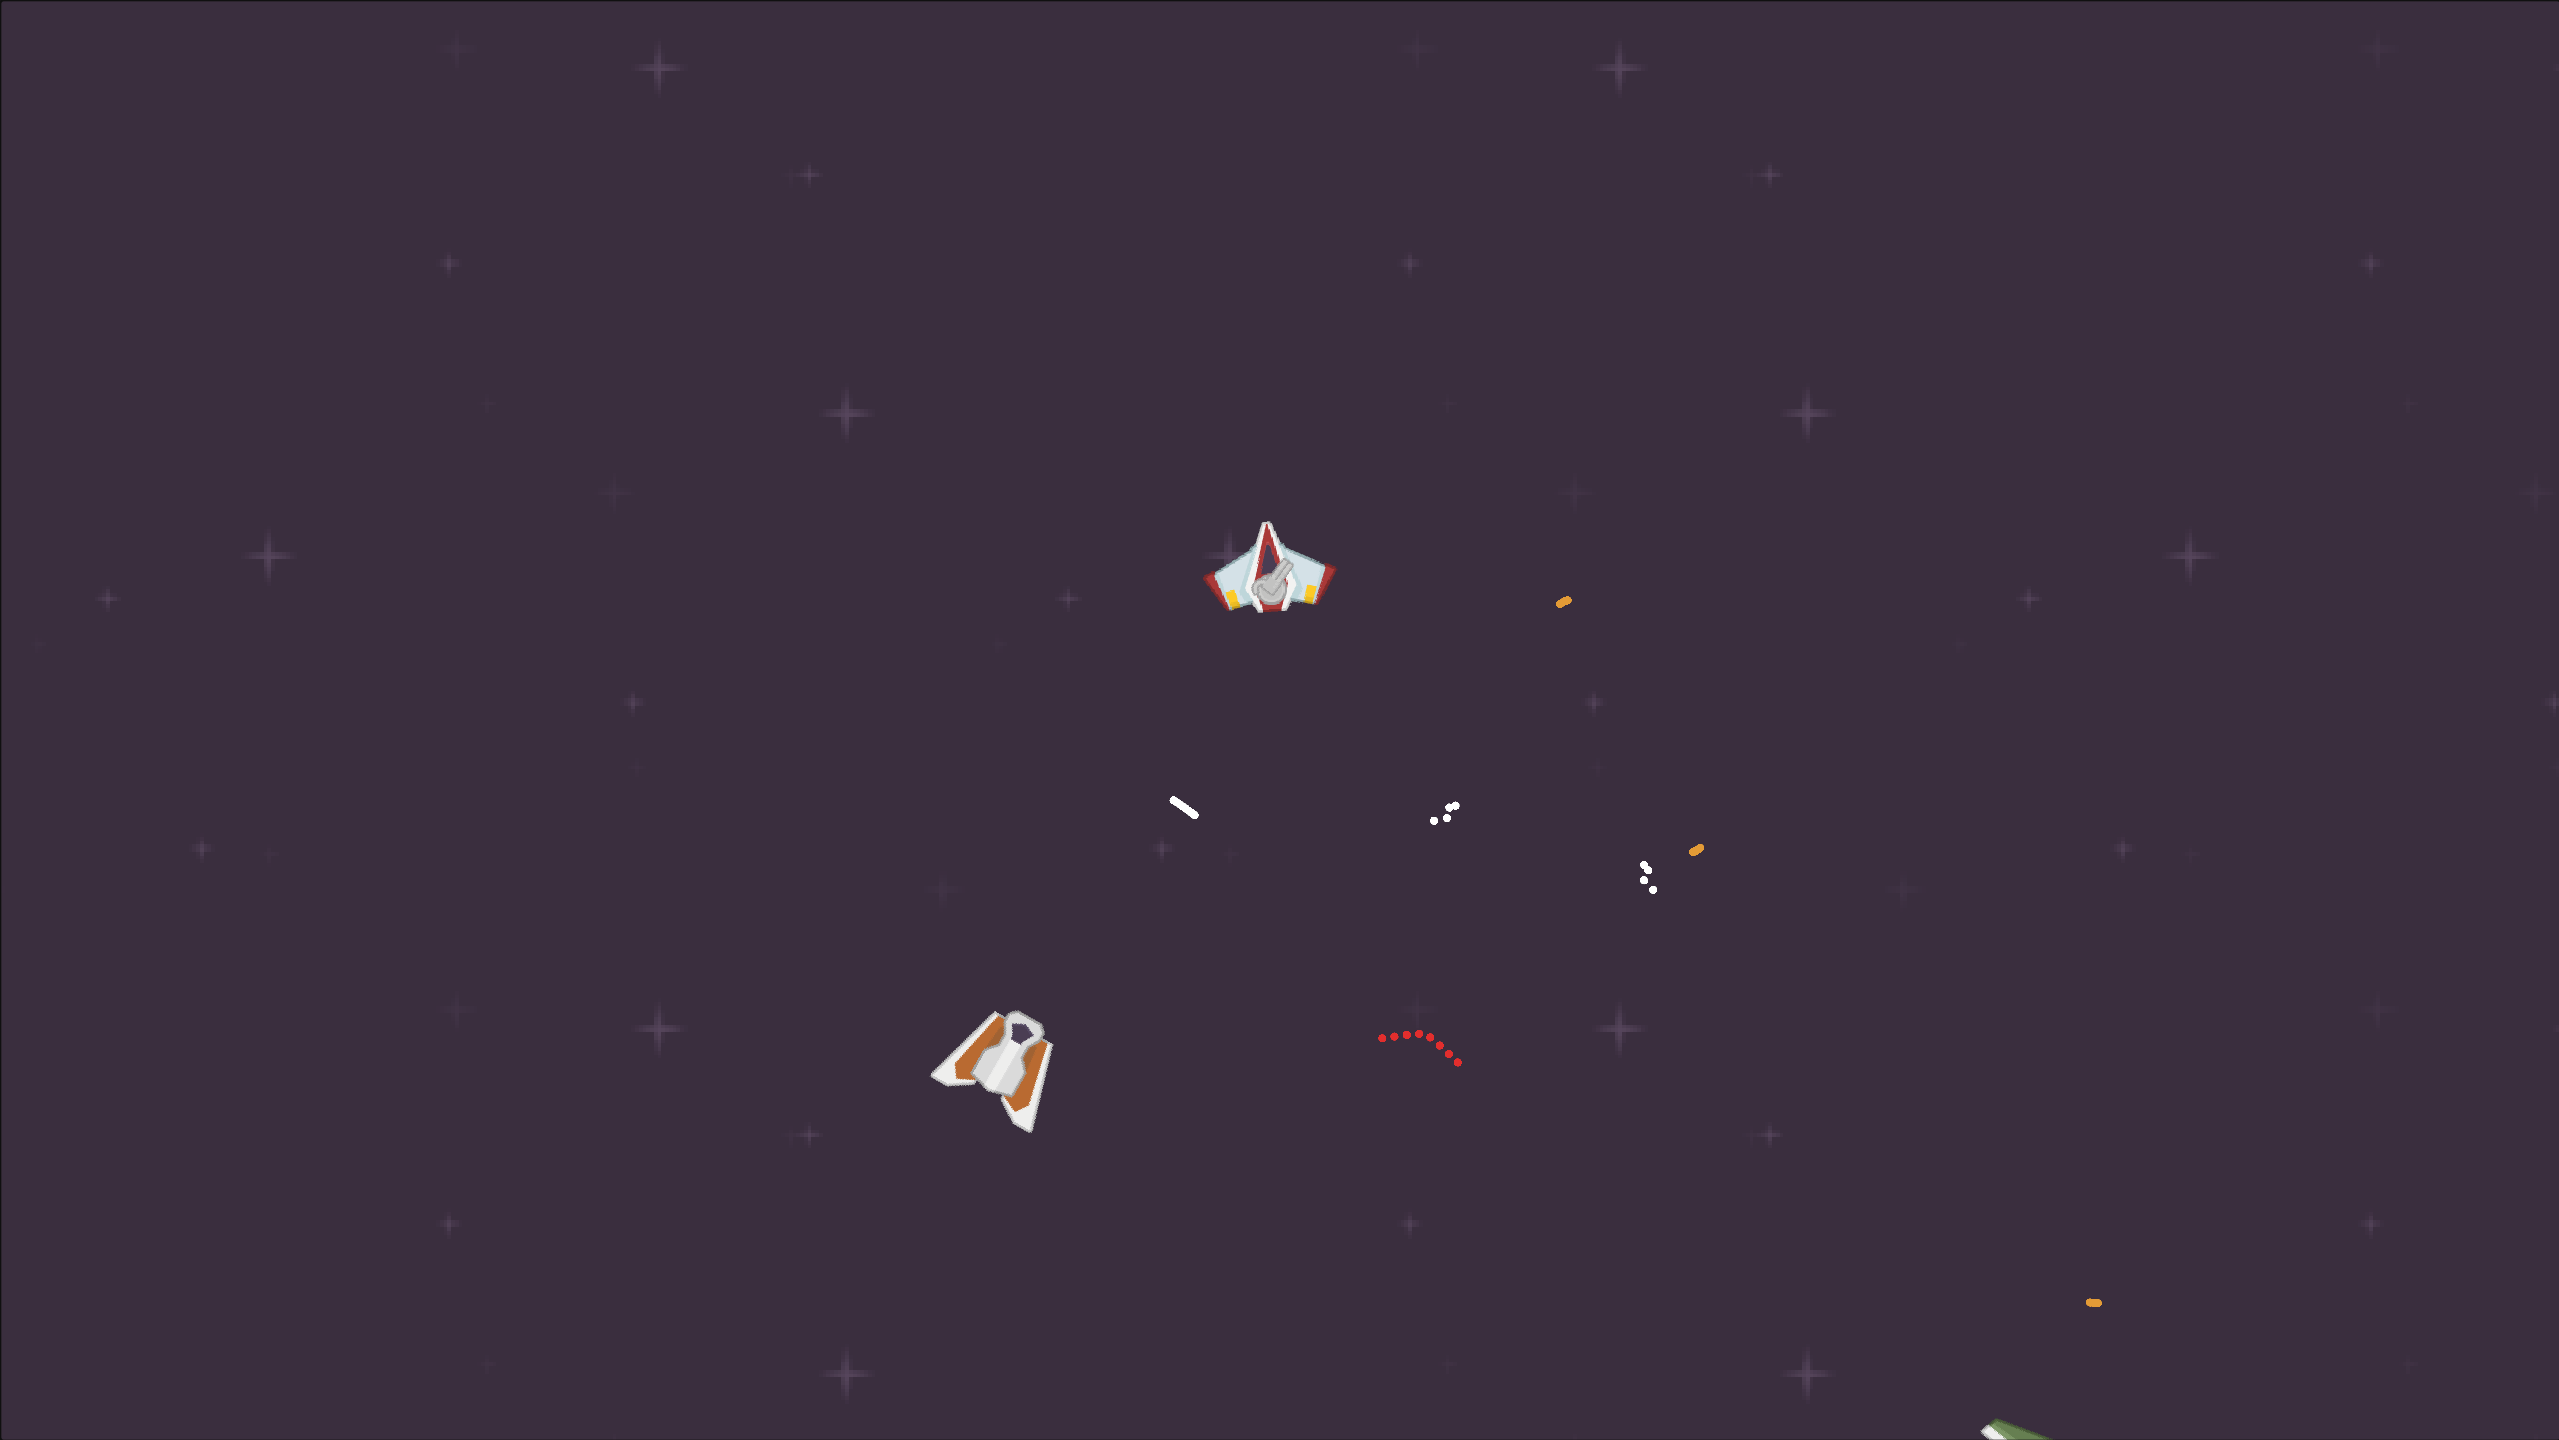
\includegraphics{images/SpaceShooter}
            }

            \caption{
                \label{SpaceShooter}
                Space Shooter.
            }
        \end {center}
    \end {figure}


\end{enumerate}

Ассеты для создания двух игр были получены с таких сайтов, как:
\begin{enumerate}
    \item Unity Asset Store\cite{s4}
    \item opengameart.org\cite{s5}
    \item itch.io\cite{s6}
\end{enumerate}

\pagebreak


\subsection{Unity Asset Store}

Для публикации было написано описание ассета, добавлены видео и скриншоты. На момент написания отчета ассет проходит модерацию.

\begin{figure}[ht]
    \begin{center}
        \scalebox{0.3}{
            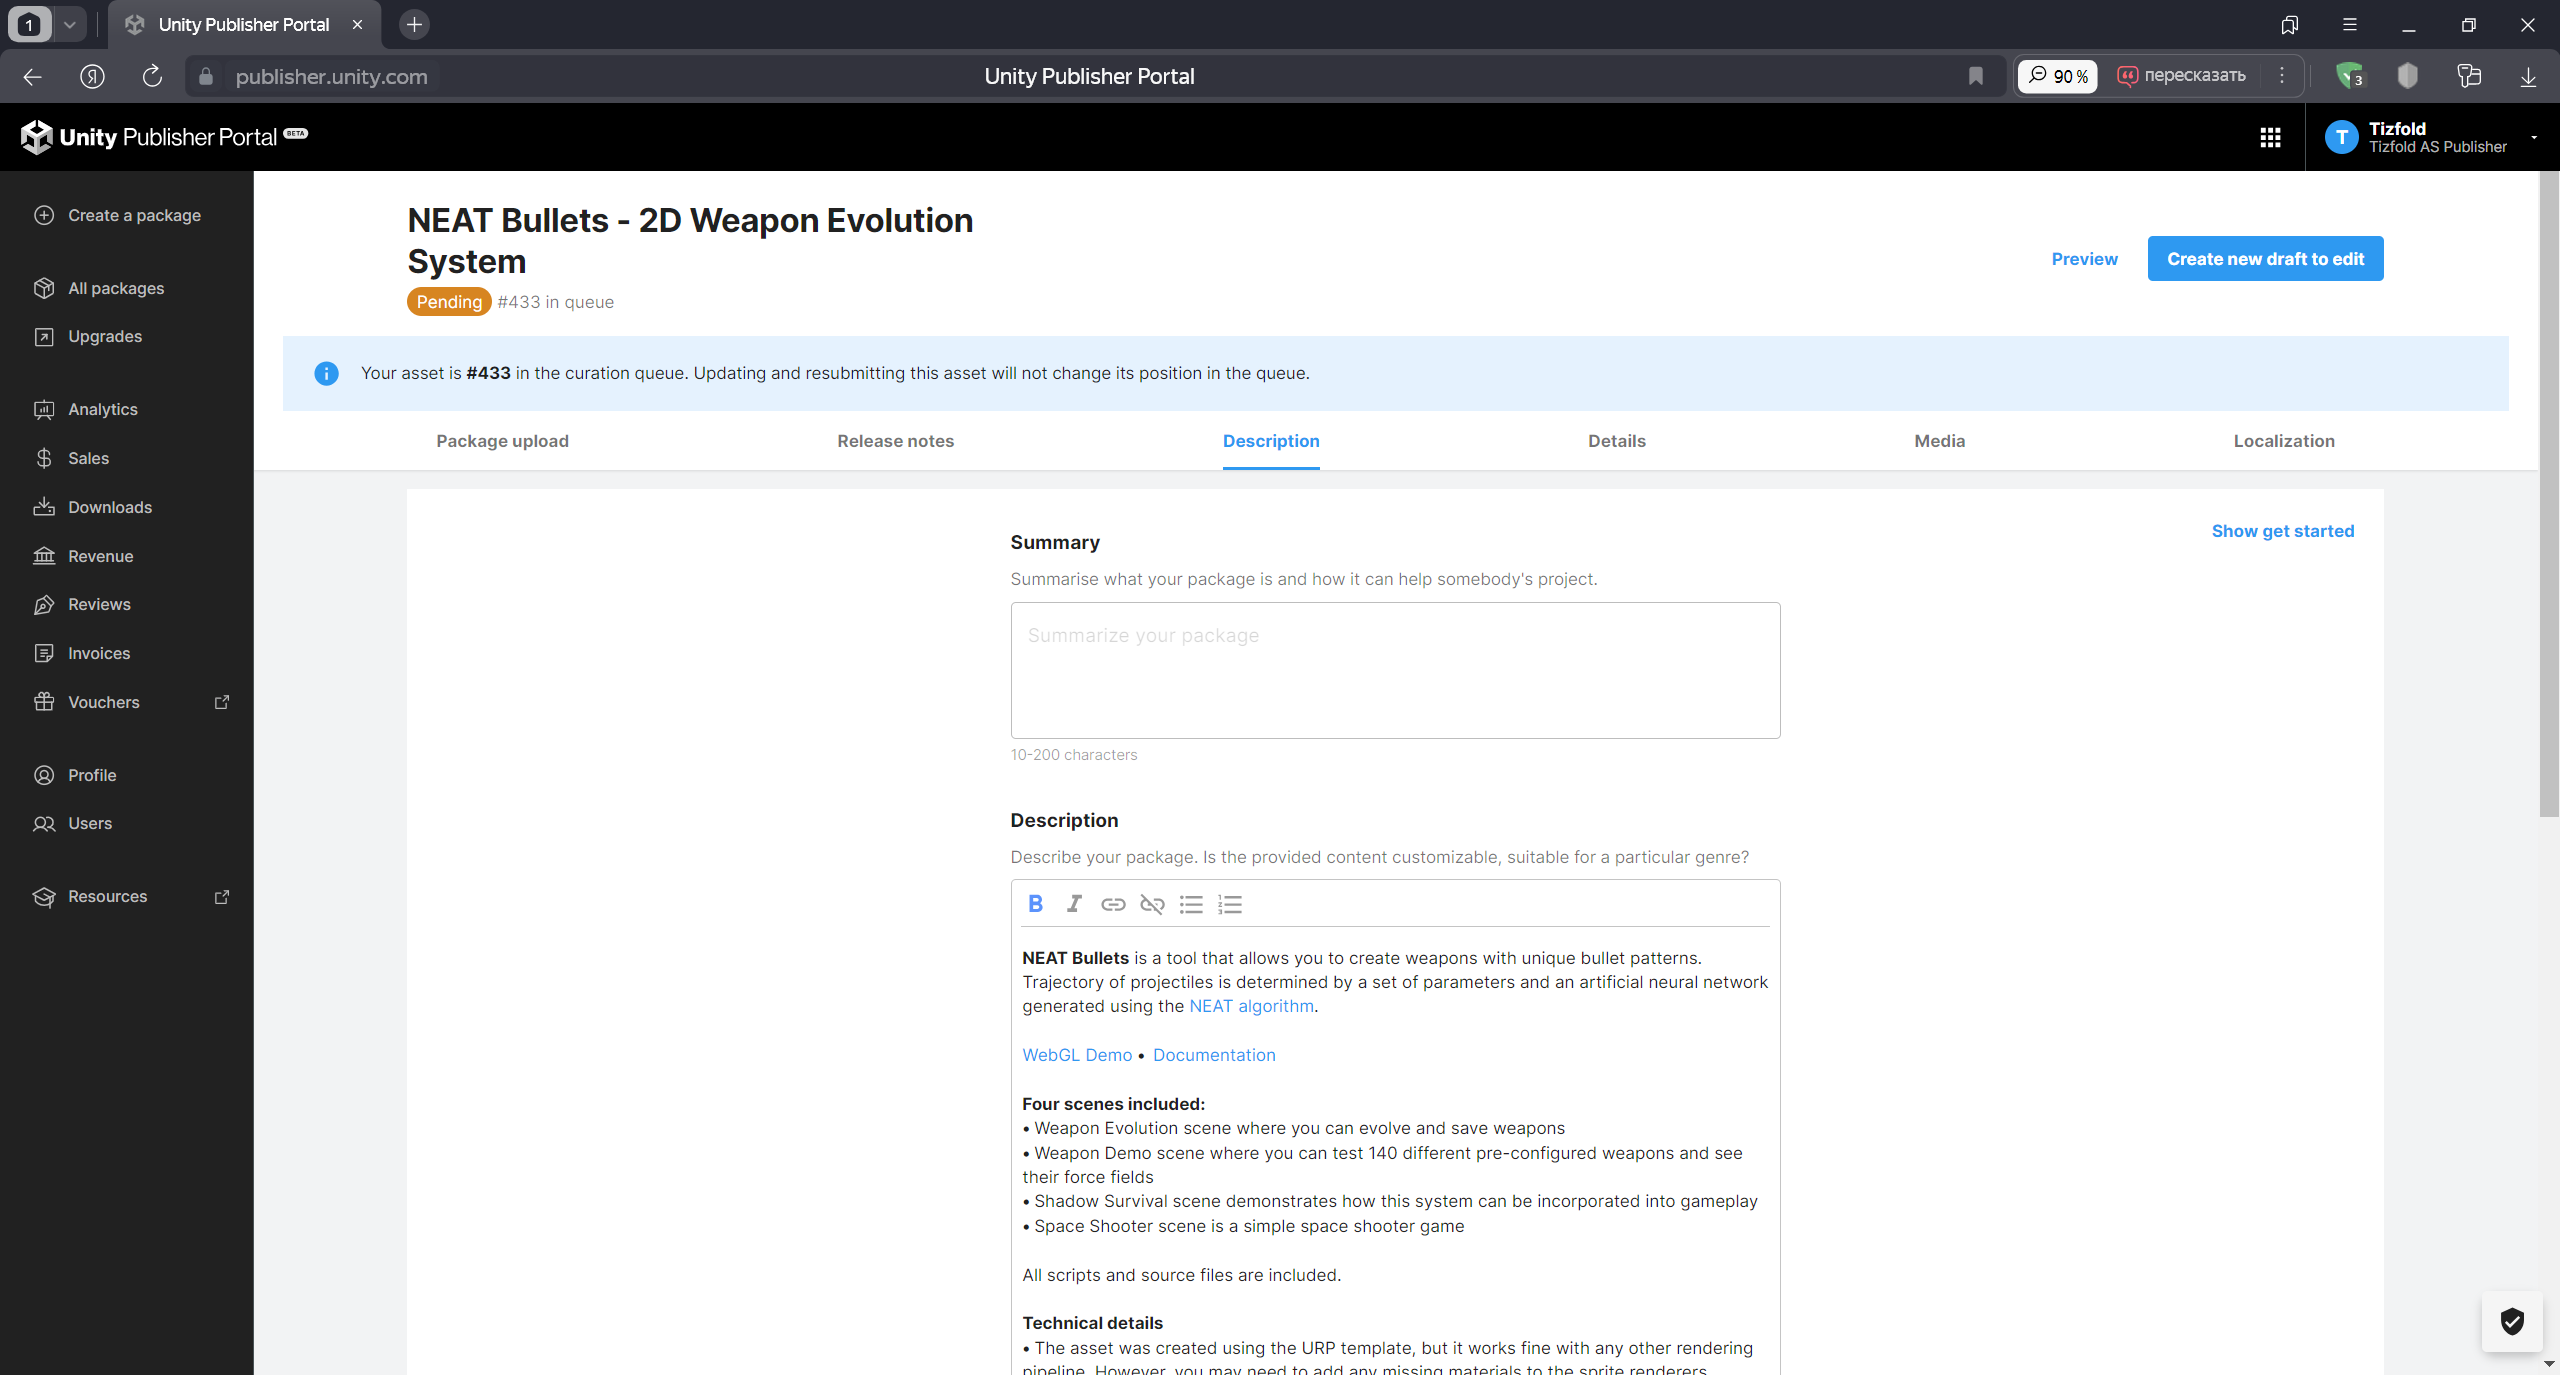
\includegraphics{images/PublisherPortal}
        }

        \caption{
            \label{PublisherPortal}
            Publisher Portal.
        }
    \end {center}
\end {figure}
\pagebreak

\specialsection{Заключение}

В результате работы были выполнены следующие задачи:

\begin{enumerate}[label=\textbullet]
    \item Были рассмотрены существующие примеры игр с процедурной генерацией оружия, отмечены плюсы и минусы их систем.
    \item Был проведён анализ популярных методов нейроэволюции и выбран наиболее оптимальный для решения поставленной задачи.
    \item Разработана система для процедурной генерации игрового оружия, которая полностью соответствует поставленным требованиям.
    \item Были найдены игровые ассеты и разработаны две простые мобильные 2D игры, показывающие применимость системы.
    \item Разработана сцена демонстрации оружия с визуализацией выводов нейронной сети в виде силового поля.
\end{enumerate}


\pagebreak

% Библиография в cpsconf стиле
% Аргумент {1} ниже включает переопределенный стиль с выравниванием слева
\begin{thebibliography}{1}

    \bibitem{s1} Kenneth O. Stanley, Risto Miikkulainen. \flqq Evolving Neural Networks through Augmenting Topologies\frqq. 2002. Available: \url{https://nn.cs.utexas.edu/downloads/papers/stanley.ec02.pdf}

    \bibitem{s2} Erin Hastings, Ratan Guha, and Kenneth O. Stanley. \flqq NEAT Particles: Design, Representation, and Animation of Particle System Effects\frqq. 2007. Available: \url{http://eplex.cs.ucf.edu/papers/hastings_cig07.pdf}

    \bibitem{s3} Erin J. Hastings, Ratan K. Guha, and Kenneth O. Stanley. \flqq Interactive Evolution of Particle Systems for Computer Graphics and Animation\frqq. 2009. Available: \url{http://eplex.cs.ucf.edu/papers/hastings_ieeetec09.pdf}

    \bibitem{s4} Unity Asset Store. Available: \url{https://assetstore.unity.com/}

    \bibitem{s5} OpenGameArt. Available: \url{https://opengameart.org/}

    \bibitem{s6} itch.io. Available: \url{https://itch.io/game-assets}

    \bibitem{s7} Репозиторий. Available: \url{https://github.com/AlexanderMenkeev/WeaponAsset}

    \bibitem{s8} SharpNEAT. Available: \url{https://github.com/colgreen/sharpneat}

    \bibitem{s9} WebGL Demo. Available: \url{https://tizfold.itch.io/neat-bullets}

    \bibitem{s10} IMGUI. Available: \url{https://docs.unity3d.com/Manual/GUIScriptingGuide.html}

    \bibitem{s11} Jekyll. Available: \url{https://jekyllrb.com/}

    \bibitem{s12} Jekyll theme Just the Docs. Available: \url{https://github.com/just-the-docs/just-the-docs}

    \bibitem{s13} NEAT Bullets documentation. Available: \url{https://alexandermenkeev.github.io/NEAT-Projectiles-docs/}

    \bibitem{s14} Borderlands wiki. Available: \url{https://borderlands.fandom.com/wiki/Borderlands_2_Weapons}

    \bibitem{s15} Paper about GAR. Available: \url{https://www.researchgate.net/publication/221157637_Evolving_content_in_the_Galactic_Arms_Race_video_game}

    \bibitem{s16} Paper about HyperNEAT. Available: \url{https://www.researchgate.net/publication/23986881_A_Hypercube-Based_Encoding_for_Evolving_Large-Scale_Neural_Networks}

    \bibitem{s17} Redzen. Available: \url{https://github.com/colgreen/Redzen}

    \bibitem{s18} log4net. Available: \url{https://github.com/apache/logging-log4net}

    \bibitem{s19} Space Shooter Redux. Available: \url{https://www.kenney.nl/assets/space-shooter-redux}

    \bibitem{s20} 5 Action Chiptunes. Available: \url{https://opengameart.org/content/5-chiptunes-action}

    \bibitem{s21} Retro Video Game Sound Effects Collection. Available: \url{https://opengameart.org/content/512-sound-effects-8-bit-style}

    \bibitem{s22} Weapon Item Icon. Available: \url{https://www.deviantart.com/viscious-speed/art/Abstract-Tiles-2-854400770}

    \bibitem{s23} Wheel Bot Dark Edition. Available: \url{https://penusbmic.itch.io/sci-fi-platformer-dark-edition}

    \bibitem{s24} Sci-Fi Samurai. Available: \url{https://penusbmic.itch.io/the-dark-series-sci-fi-samurais}

    \bibitem{s25} Top down dungeon tileset. Available: \url{https://opengameart.org/content/top-down-dungeon-tileset}

\end{thebibliography}
\pagebreak

\specialsection{Приложение}\label{sec:appendix}

\begin{lstlisting}[caption={Пример XML файла, представляющего некоторую нейронную сеть},label={lst:xml}]
<?xml version="1.0" encoding="utf-8"?>
<Root>
  <ActivationFunctions>
    <Fn id="0" name="Linear" prob="0.1" />
    <Fn id="1" name="Sine" prob="0.1" />
    <Fn id="2" name="ArcTan" prob="0.1" />
    <Fn id="3" name="BipolarGaussian" prob="0.1" />
    <Fn id="4" name="BipolarSigmoid" prob="0.1" />
    <Fn id="5" name="LogisticFunction" prob="0.1" />
    <Fn id="6" name="QuadraticSigmoid" prob="0.1" />
    <Fn id="7" name="TanH" prob="0.1" />
    <Fn id="8" name="ArcSinH" prob="0.1" />
    <Fn id="9" name="ReLU" prob="0.1" />
  </ActivationFunctions>
  <Networks>
    <Network id="2" birthGen="0" fitness="0">
      <Nodes>
        <Node type="bias" id="0" fnId="0" />
        <Node type="in" id="1" fnId="0" />
        <Node type="in" id="2" fnId="0" />
        <Node type="in" id="3" fnId="0" />
        <Node type="out" id="4" fnId="0" />
        <Node type="out" id="5" fnId="0" />
        <Node type="out" id="6" fnId="0" />
        <Node type="out" id="7" fnId="0" />
        <Node type="out" id="8" fnId="0" />
      </Nodes>
      <Connections>
        <Con id="9" src="0" tgt="4" wght="-1.2483117076970207" />
        <Con id="10" src="0" tgt="5" wght="1.2919574609799234" />
        <Con id="11" src="0" tgt="6" wght="3.2976727814611015" />
        <Con id="12" src="0" tgt="7" wght="4.5639186117631994" />
        <Con id="13" src="0" tgt="8" wght="1.6772187331988953" />
        <Con id="14" src="1" tgt="4" wght="-2.5150411873873879" />
        <Con id="15" src="1" tgt="5" wght="1.6835215086014244" />
        <Con id="16" src="1" tgt="6" wght="-3.0142861092056847" />
        <Con id="17" src="1" tgt="7" wght="-4.8501571712828042" />
        <Con id="18" src="1" tgt="8" wght="-4.9350933966085018" />
        <Con id="19" src="2" tgt="4" wght="-0.861845813939025" />
        <Con id="20" src="2" tgt="5" wght="4.8588766566951609" />
        <Con id="21" src="2" tgt="6" wght="3.3680268141368774" />
        <Con id="22" src="2" tgt="7" wght="-4.8566069123074351" />
        <Con id="23" src="2" tgt="8" wght="1.987358882250988" />
        <Con id="24" src="3" tgt="4" wght="2.8582354891729009" />
        <Con id="25" src="3" tgt="5" wght="-0.83853102580048411" />
        <Con id="26" src="3" tgt="6" wght="3.8769237625958466" />
        <Con id="27" src="3" tgt="7" wght="-0.1136256214976461" />
        <Con id="28" src="3" tgt="8" wght="4.1622872269401165" />
      </Connections>
    </Network>
  </Networks>
</Root>
\end{lstlisting}


\begin{lstlisting}[caption={Пример json файла с параметрами некоторого оружия},label={lst:json}]
{
    "<WeaponMode>k__BackingField": 0,
    "<BurstMode>k__BackingField": 2,
    "<BurstRate>k__BackingField": 0.05000000074505806,
    "<FireRate>k__BackingField": 0.30000001192092898,
    "<ProjectilesInOneShot>k__BackingField": 4,
    "<RotationSpeed>k__BackingField": 0.0,
    "<MoveSpeed>k__BackingField": 10.0,
    "<NetworkControlMode>k__BackingField": 0,
    "<ReadMode>k__BackingField": 0,
    "<Size>k__BackingField": {
        "x": 0.07000000029802323,
        "y": 0.07000000029802323
    },
    "<HasLifespan>k__BackingField": true,
    "<Lifespan>k__BackingField": 8.0,
    "<HasTrail>k__BackingField": true,
    "<HueRange>k__BackingField": {
        "x": 0.4115835428237915,
        "y": 0.7891817092895508
    },
    "<Saturation>k__BackingField": 0.8029999732971191,
    "<Brightness>k__BackingField": 1.0,
    "<SpeedRange>k__BackingField": {
        "x": 2.5092172622680666,
        "y": 5.50921630859375
    },
    "<ForceRange>k__BackingField": {
        "x": 1.4973399639129639,
        "y": 3.4973397254943849
    },
    "<NNControlDistance>k__BackingField": 4.0,
    "<SignX>k__BackingField": 0.0,
    "<SignY>k__BackingField": -1.0,
    "<ForwardForce>k__BackingField": false,
    "<InitialFlightRadius>k__BackingField": 0.05000000074505806,
    "<InitialSpeed>k__BackingField": 0.5,
    "<Angle>k__BackingField": 179.0,
    "<FlipXOnReflect>k__BackingField": false,
    "<FlipYOnReflect>k__BackingField": false,
    "<Mode>k__BackingField": 0,
    "<ReflectiveCircleRadius>k__BackingField": 1.4142135381698609,
    "<RectDimensions>k__BackingField": {
        "x": 1.0,
        "y": 1.0
    },
    "<MaxPolarAngleDeg>k__BackingField": 65.0
}
\end{lstlisting}






\end{document}